\documentclass[conference,onecolumn,oneside]{IEEEtran}
\IEEEoverridecommandlockouts
\usepackage[space]{grffile}
\usepackage{cite}
\usepackage{amsmath,amssymb,amsfonts}
\usepackage{graphicx}
\usepackage{textcomp}
\usepackage{xcolor}
\usepackage{float}
\usepackage{titlesec}
\usepackage{tocloft}
\usepackage{caption}
\captionsetup[figure]{labelfont=bf}
\pagestyle{plain}
\usepackage{subcaption}
\usepackage{svg}\usepackage{svg}
\usepackage{setspace}
\usepackage{verbatim}
\usepackage{tcolorbox}
\tcbuselibrary{skins,breakable}
\doublespacing
\usepackage{multirow}
\usepackage{hyperref}
\hypersetup{
    colorlinks=true,
    linkcolor=black,
    citecolor=blue,
    urlcolor=blue
}
\renewcommand{\cfttoctitlefont}{\Huge\bfseries\color[rgb]{0.16, 0.24, 0.5}}
\renewcommand{\contentsname}{Contents}
\renewcommand{\thesection}{\arabic{section}}
\renewcommand{\thesubsection}{\thesection.\arabic{subsection}}
\renewcommand{\thesubsubsection}{\thesubsection.\arabic{subsubsection}}
\titleformat{\section}
  {\normalfont\Large\bfseries}{\thesection}{1em}{}
\titleformat{\subsection}
  {\normalfont\large\bfseries}{\thesubsection}{1em}{}
\renewcommand{\cftsecfont}{\bfseries}
\renewcommand{\cftsecleader}{\cftdotfill{\cftdotsep}}
\renewcommand{\cftsecpagefont}{\bfseries}
\begin{document}
\begin{titlepage}
    \begin{center}
        \vspace*{1cm}
        \huge \textbf{PosePulse: Multi-Task Exercise Analysis with Classification, Quality Scoring, and Coaching Feedback}
        \vspace{2.5cm}

        \large Author \\
        \Large \textbf{Elina Melkonyan}

        \vspace{1.5cm}
        \large Supervised by \\
        \Large \textbf{Hermine Grigoryan}

        \vfill
        \includegraphics[width=0.4\textwidth]{AUA_official_logo.png} \\
        \large American University of Armenia

        \vspace{1.5cm}
        \large A Capstone submitted in partial fulfillment of requirements for the degree of \\
        Bachelor of Science in Computer Science

        \vspace{0.8cm}
        \large Akian College of Science and Engineering \\
        American University of Armenia \\
        May 2026
    \end{center}
\end{titlepage}

\section*{Abstract}
\begin{quotation}
\itshape
The fitness industry faces a costly paradox: while beginners pay premium prices for online coaches, they often receive delayed, generic feedback on exercise form. This lack of real-time correction is more than an inefficiency; the consistent, repetitive execution of exercises with improper biomechanics is the primary driver of chronic training injuries. Whether relying on subjective self-assessment in mirrors or expensive remote coaching, trainees lack the immediate, biomechanically accurate guidance necessary to ensure safe execution.
To address this issue, this paper proposes PosePulse, a computer vision system for real-time exercise classification and execution-quality assessment from monocular RGB video.  PosePulse first compares a BiLSTM-CNN baseline against an xLSTM backbone on the exercise classification task. The xLSTM encoder is then extended into a multi-task model trained on EgoExo-Fitness dataset, where a single shared encoder simultaneously predicts movement quality, generates a clip-specific coaching comment, and retrieves the corresponding exercise guidance --- turning a classifier into a feedback system that addresses both what the user is doing and how to improve it.
The results demonstrate that a lightweight, retrieval-based pipeline
can deliver meaningful coaching feedback without large-scale generative
components, making real-time deployment on consumer hardware a
realistic near-term goal.
\vspace*{0.3cm}
\textbf{Index Terms---} Pose Estimation, BiLSTM, xLSTM, Exercise Classification,
Action Quality Assessment, Multi-Task Learning, Biomechanics.
\end{quotation}
\newpage
\vspace*{1cm}
\tableofcontents
\newpage

\section{Introduction}
\vspace*{1cm}
\subsection{Motivation}
\vspace{0.5cm}
Improper exercise technique is one of the leading causes of training-related injury. Studies in sports medicine consistently show that a significant proportion of gym-related injuries can be attributed not to the exercise itself but to poor joint alignment, insufficient range of motion, or compensatory movement patterns that place excessive stress on passive structures such as ligaments and intervertebral discs. This risk has intensified considerably with the rise of social media fitness culture. Platforms such as TikTok, Instagram, and YouTube have made workout content more accessible than ever, motivating millions of users to attempt exercises independently and without professional oversight. Yet this democratization of fitness carries a structural hazard: many fitness influencers lack formal training and may demonstrate incorrect techniques, leading to improper posture, excessive joint stress, and elevated injury risk. Without any mechanism to verify whether the viewer is replicating a movement correctly, the gap between watching an exercise and safely executing it remains entirely unmediated.
Recent advances in computer vision and deep learning have unlocked practical solutions to the problem of automated exercise analysis. Pose estimation frameworks - which extract skeletal joint coordinates from monocular RGB video at real-time frame rates - have become central to this effort, enabling downstream systems to reason about body configuration without specialized hardware. Combining pose estimation with sequence classification models has enabled systems that can identify which exercise is being performed and evaluate the quality of its execution. Critically, unlike raw pixel-based approaches, skeleton representations generalize across users, lighting conditions, and camera viewpoints, making them well-suited for deployment on consumer-grade devices~\cite{1}.
Standard recurrent architectures such as vanilla RNNs and conventional LSTMs have long served as the default choice for temporal sequence modeling in action recognition tasks, with LSTM-based approaches widely adopted to handle lengthy action sequences. Vanilla RNNs effectively incorporate short-term temporal dependencies, and CNN-RNN hybrid architectures have demonstrated substantial improvements in video classification accuracy across multiple benchmark datasets~\cite{16},~\cite{3}. However, when applied to the dual demands of exercise classification and quality assessment, their structural limitations become directly consequential.
These limitations have driven the field toward Transformer-based architectures. Transformers, with their self-attention mechanism, address the parallelization and long-range dependency problems that cripple standard LSTMs --- however, they require large amounts of data and computational resources, and their quadratic complexity with respect to sequence length makes them less suitable for real-time deployment on resource-constrained devices~\cite{4}.  Rather than adopting a Transformer backbone, PosePulse follows the direction proposed by Beck et al.\cite{4}, which extends the LSTM architecture with exponential gating and new memory structures and demonstrates that xLSTM compares favorably to Transformers and state-space models in terms of both performance and scaling laws.\cite{4}

\vspace{0.5cm}
\subsection{Problem statement and objectives}
\vspace{0.5cm}
PosePulse targets a gap that existing fitness applications have not
closed: the simultaneous, automated analysis of what a user is doing
and how correctly they are doing it, delivered from nothing more than
a standard monocular camera. The paper pursues two objectives to close
this gap.

\textbf{Backbone comparison for exercise classification.}
The first objective is to evaluate whether xLSTM --- a recently
proposed recurrent architecture with exponential gating and matrix
memory --- offers advantages over a BiLSTM--CNN baseline for exercise
classification from skeletal features. The comparison is conducted
across three feature conditions (hand-crafted joint angles and
coordinates, ResNet-50 appearance embeddings, and ViTPose-S pose
embeddings) to determine whether any performance advantage is
architecture-driven or feature-dependent.

\textbf{Multi-task quality assessment and coaching feedback.}
Classification alone is insufficient for coaching purposes. The second
objective is to extend the xLSTM encoder into a multi-task model that
simultaneously predicts movement quality, retrieves a clip-specific
coaching comment, and provides an exercise-level guidance string ---
turning a classifier into a feedback loop that tells the user both
what they are doing and how to improve it. This objective is pursued
on the EgoExo-Fitness dataset, whose interpretable action-judgement
annotations furnish the continuous quality scores and natural-language
comments required for supervision. The coaching comment is retrieved
from a parameter-free lookup table conditioned on the predicted
exercise class and quality bucket, rather than generated; this is a
deliberate choice dictated by the limited annotation density of the
EgoExo-Fitness corpus, and the architecture is designed to accommodate
a lightweight generative decoder as larger annotated datasets become
available.

\vspace{1.0cm}

\section{Literature review}
\vspace{0.75cm}
\subsection{Existing approaches}
\vspace{0.5cm}
\textbf{CNN-based approaches:}
The earliest attempts at automated exercise analysis did not involve learning at all --- they compared what the user was doing against fixed references and flagged deviations that exceeded predefined thresholds~\cite{9},~\cite{10}. Dsouza et al.~\cite{9} aligned user movements to reference videos through DTW, using VGG-19 for feature extraction and CNNs for body part mapping, evaluated on a self-collected dataset of indoor workout videos recorded under controlled laboratory conditions. Chen and Yang~\cite{10} computed joint angles and torso-normalized distances against trainer-defined thresholds, supplemented by a DTW nearest-neighbor classifier that returned a binary correct/incorrect verdict, trained and tested on a self-recorded dataset of approximately 100 videos covering four dumbbell exercises. Nagarkoti et al.~\cite{11} used CNNs to localize joints and evaluate performance against professional athlete benchmarks through heuristic rule-based comparisons. Bang and Park~\cite{12} trained a CNN ensemble on MediaPipe-extracted joint coordinates and angles for real-time exercise classification, achieving 92.12\% classification accuracy on their test set. However, these CNN-based and DTW-based approaches share a fundamental limitation: they operate on individual frames or fixed templates without modeling how a movement unfolds over time.
\textbf{LSTM and GCN-Based Approaches:}
The shortcomings of frame-level methods led the field toward architectures capable of modeling temporal dynamics. Alatiah and Chen~\cite{13} proposed a stacked LSTM trained on 8-frame sequences of BlazePose (x, y, z) coordinates, which achieved real-time classification but was sensitive to camera distance. Riccio~\cite{1} addressed this directly by training a BiLSTM on 30-frame windows of combined joint angles and (x, y, z) coordinates, achieving over 99\% classification accuracy on the test set.
On the graph-based side, Deb et al.~\cite{14} adapted ST-GCN to predict continuous rehabilitation quality scores from 3D skeleton sequences. Similarly, a multi-task ST-GCN variant~\cite{15} extended this to gym exercises. While GCN-based approaches are a step forward, they typically require 3D skeleton inputs from depth sensors, which are not available in standard monocular webcam deployments. PosePulse responds by evaluating xLSTM \cite{4} as its primary backbone, specifically adopting the xLSTM[7:1] configuration (7 mLSTM + 1 sLSTM blocks) identified as optimal for long-sequence modeling as its core sequence modeling backbone.~\cite{4}
\begin{figure}[H]
    \centering
    \includegraphics[width=\linewidth, height =8cm]{xlstm_struct.png}
    \caption{\textbf{The extended LSTM (xLSTM) family.} From left to right: 1. The original LSTM memory cell with constant error carousel and gating. 2. New sLSTM and mLSTM memory cells that introduce exponential gating. sLSTM offers a new memory mixing technique. mLSTM is fully parallelizable with a novel matrix memory cell state and new covariance update rule. 3. mLSTM and sLSTM in residual blocks yield xLSTM blocks. 4. Stacked xLSTM blocks give an xLSTM architecture. Reproduced by \cite{4}}
    \label{fig:placeholder}
\end{figure}
Unlike prior LSTM variants that struggled with vanishing gradients over 30-frame exercise windows, xLSTM's matrix memory (mLSTM) maintains separable state representations for both exercise classification and quality assessment within the same shared encoder, while its exponential gating ensures stable gradients.~\cite{4} Critically, this architecture matches Transformer parallelization while eliminating their quadratic complexity, enabling real-time inference on consumer hardware perfectly suited for embedded and edge applications due to its speed and low, constant memory footprint.~\cite{4}

\vspace{0.5cm}
\subsection{Existing datasets}
\vspace{0.5cm}
The development of robust and generalizable exercise analysis models relies heavily on the availability of high-quality, annotated video datasets that capture both exercise identity and execution quality. However, datasets that satisfy both requirements simultaneously are relatively scarce compared to general action recognition benchmarks in computer vision.
Several datasets have been proposed to address different facets of this problem. Fitness-AQA, introduced by Parmar et al. at ECCV 2022 ~\cite{7}, covers three barbell exercises:  BackSquat, BarbellRow, and OverheadPress which have been annotated by expert trainers for multiple commonly occurring execution errors. While Fitness-AQA was the first fitness-specific quality assessment dataset, its annotation scheme is binary rather than continuous, and its exercise coverage is limited to three barbell movements.
Fit3D ~\cite{8} takes a different approach, providing over 3 million images and corresponding 3D pose configurations for 37 fitness exercises across various skill levels, captured using 12 synchronized motion capture cameras. However, its controlled laboratory capture conditions and fixed camera viewpoints make it poorly representative of the uncontrolled environments encountered in real-world home and gym deployments. More recently, FLEX ~\cite{6} introduces the first large-scale, multimodal dataset for fitness action quality assessment, containing over 7,500 multi-view recordings of 20 weight-loaded exercises performed by 38 subjects across three skill levels, with synchronized RGB video, 3D pose, surface electromyography signals, and physiological data.
\begin{figure}[H]
    \centering
    \includegraphics[width=0.7\linewidth, height = 8cm]{Screenshot 2026-05-02 at 16.40.05.png}
    \caption{\textbf{An overview of the FLEX dataset.} FLEX dataset consists of a core group of 38 subjects, each performing 20 different fitness actions, repeating each action 10 times. Each action repeat was recorded from 5 viewpoints, \& sEMG signals and physiological parameters (heart rate, breath rate) were simultaneously collected along with videos. The data annotations contain rich text information such as action keysteps (AK), error types (ET), \& action feedback. Reproduced by~\cite{6}}
    \label{fig:placeholder}
\end{figure}
\begin{figure}[H]
    \centering
    \includegraphics[width=1\linewidth]{Screenshot 2026-05-01 at 00.40.43.png}
    \caption{\textbf{An overview of Riccio dataset.} Images from the Datasets used for training and validation of the exercise classifier. (images are cropped due to screenshots, hence they appear to have different dimensions) Reproduced by~\cite{1}}
    \label{fig:riccio_dataset}
\end{figure}
To address the classification task, PosePulse draws on the dataset compiled by Riccio ~\cite{6}, which combines synthetic data from the InfiniteRep dataset with real-world videos sourced from the Kaggle Workout/Exercises Video Dataset. This combination was chosen specifically to ensure robustness across the diverse conditions encountered outside controlled laboratory settings with varying lighting, camera angles, and subject body types. However, this dataset provides only exercise-type labels and contains no annotations regarding execution quality, making it insufficient as a standalone resource for training the quality assessment head.
To extend PosePulse beyond exercise identification toward biomechanically grounded coaching feedback, we leverage the EgoExo-Fitness dataset~\cite{2}. The core dataset consists of a comprehensive multimodal corpus explicitly annotated for action evaluation:
\begin{itemize}
    \item \textbf{Dataset Scale:} It contains a total of 1,525 segmented video clips derived from 137 long-form fitness execution recordings.
    \item \textbf{Subject Diversity:} The execution data spans 41 unique human subjects performing movements across varying physical capabilities and skill levels.
    \item \textbf{Exercise Coverage:} The annotations encompass 12 distinct functional fitness action classes, including both upper-body, lower-body, and compound movements.
    \item \textbf{Annotation Density:} A total of 4,374 dense judgment pairs provide temporal boundaries, technical keypoint verifications, clip-specific natural language coaching feedback, and scalar quality scores.
\end{itemize}
These interpretable action judgment annotations directly furnish the three supervision signals required for our multi-task pipeline: a continuous quality score ($\text{action\_quality\_score} \in \{1, \ldots, 5\}$), a clip-specific natural-language coaching comment written by expert annotators, and an exercise-level action guidance string recommending biomechanical instructions.
An empirical inspection of the 1,525 annotated clips reveals that the \texttt{action\_guidance} string is class-deterministic: every clip of a given exercise carries an identical guidance text, while the \texttt{comment} field is clip-specific and varies with the observed execution quality.
\begin{figure}[H]
    \centering
    \includegraphics[width=1\linewidth]{Screenshot 2026-05-01 at 00.46.57.png}
    \caption{\textbf{An Overview of EgoExo-Fitness.} (a) The dataset features synchronized egocentric and exocentric videos of fitness activities to support future work on egocentric full-body action understanding. (b) EgoExo-Fitness provides abundant annotations, including two-level temporal boundaries and interpretable action judgment. (c) They benchmark EgoExo-Fitness on five relevant tasks. Reproduced by~\cite{2}}
    \label{fig:placeholder}
\end{figure}

\vspace*{0.8cm}

\section{Methodology}
\vspace*{0.5cm}
\subsection{Comparison of Human Skeleton Extraction Frameworks}
\vspace{0.5cm}
Selecting an appropriate pose estimation backbone is a foundational decision for PosePulse, since the quality, consistency, and speed of extracted features directly determines the reliability of all downstream angle computation, sequence modeling, and quality scoring. To make this selection empirically rather than arbitrarily, a systematic comparison was conducted across five pose estimation frameworks on a controlled subset of the target data.

\vspace{0.3cm}
\subsubsection{Candidate Pose Estimation Backends}
\vspace{0.3cm}
The following frameworks were selected to span the range from lightweight mobile-optimized models to state-of-the-art transformer-based estimators:
\begin{itemize}
    \item \textbf{MediaPipe BlazePose:} Google's mobile-optimized framework predicting 33 keypoints, chosen as a widely adopted fitness baseline~\cite{17}.
    \item \textbf{MoveNet Lightning:} A lightweight, high-speed convolutional model from Google designed specifically for tracking fitness and yoga poses, capable of sub-10ms inference on most consumer hardware~\cite{18}.
    \item \textbf{RTMPose:} A high-performance real-time framework using a CSPNeXT backbone, designed for efficient 2D human pose estimation across various deployment scenarios~\cite{19}.
    \item \textbf{YOLOv8-Pose:} A single-stage CNN detector following the 17-keypoint COCO topology, offering a robust balance between inference speed and detection accuracy~\cite{20}.
    \item \textbf{ViTPose:} A plain vision transformer backbone equipped with a lightweight decoder, representing the current state-of-the-art accuracy frontier for 2D pose estimation~\cite{21}.
    \item \textbf{DETRPose:} The first end-to-end real-time transformer model for multi-person pose estimation, released in 2025 to address complex spatial relationships between joints~\cite{22}.
\end{itemize}

\subsubsection{Experimental Setup}
\vspace{0.3cm}
To ensure a rigorous and unbiased comparison, thirty videos were randomly sampled from the Riccio dataset~\cite{1}, covering all four target exercise classes: squat, push-up, shoulder press, and bicep curl. The sampling strategy ensured a balanced representation across different subjects, camera distances, and various lighting conditions to simulate real-world training environments. Each framework was executed on identical hardware under uniform background load conditions.
The performance of each backbone was evaluated across four primary metrics chosen to reflect the practical constraints of a real-time consumer deployment:
\begin{itemize}
    \item \textbf{FPS (Frames Per Second):} Measured the throughput during live inference. This metric is critical for determining whether the system can sustain continuous feedback without frame drops that would disrupt the user experience.
    \item \textbf{Latency (ms):} Calculated the per-frame processing delay. This determines the responsiveness of the corrective feedback; lower latency is essential for preventing the ``lag'' effect between user movement and system reaction.
    \item \textbf{Keypoint Confidence:} The mean confidence score produced by the model across the 17 body joints. This reflects detection reliability, particularly under the high-occlusion and motion-blur conditions common during rapid exercise repetitions.
    \item \textbf{Detection Rate:} The proportion of total frames in which all required joints were successfully localized. This metric reflects the robustness of the framework across the full movement arc of an exercise.
\end{itemize}
\begin{figure}
    \centering
    \includegraphics[width=0.8\linewidth]{combined_all_exercises.png}
    \caption{Multi-backend qualitative skeleton overlays on three sampled frames of a single Riccio exercise clips (rows = backends, columns = time; COCO-17, confidence threshold 0.3 for counting visible joints).}
    \label{fig:skeleton_grid_panels_full}
\end{figure}
\begin{figure}[H]
    \centering
    \begin{subfigure}[b]{0.45\linewidth}
        \centering
        \includegraphics[width=\linewidth]{comparison_summary_biceps.png}
        \caption{Biceps curl}
    \end{subfigure}
    \hfill
    \begin{subfigure}[b]{0.45\linewidth}
        \centering
        \includegraphics[width=\linewidth]{comparison_summary_shoulderpress.png}
        \caption{Shoulder press}
    \end{subfigure}
\end{figure}
\begin{figure}[H]
    \ContinuedFloat
    \centering
    \begin{subfigure}[b]{0.45\linewidth}
        \centering
        \includegraphics[width=\linewidth]{comparison_summary_squat.png}
        \caption{Squat}
    \end{subfigure}
    \hfill
    \begin{subfigure}[b]{0.45\linewidth}
        \centering
        \includegraphics[width=\linewidth]{comparison_summary_pushup.png}
        \caption{Push-up}
    \end{subfigure}
    \caption{\textbf{Per-exercise pose backend benchmark (Riccio).} For each exercise stratum, N clips were sampled at random (fixed seed). Each backend was run on the same clips; bars report mean throughput (FPS), mean per-frame latency (ms), mean joint confidence ($\times100$), and detection rate. The text panel lists the best backend per metric and the balanced choice obtained by summing min--max-normalised FPS, confidence, and detection rate across backends on that stratum.}
\end{figure}
To determine the final pose estimation backbone, a composite score
$S_m$ was computed for each framework $m \in \mathcal{M}$ by
min--max normalising the three primary metrics --- mean FPS $f_m$,
mean keypoint confidence $c_m$, and detection rate $d_m$ --- across
all models in the benchmark, then summing the normalised values:
\begin{equation}
\tilde{f}_m = \frac{f_m - \min_{k} f_k}{\max_{k} f_k - \min_{k} f_k + \varepsilon},
\quad
\tilde{c}_m = \frac{c_m - \min_{k} c_k}{\max_{k} c_k - \min_{k} c_k + \varepsilon},
\quad
\tilde{d}_m = \frac{d_m - \min_{k} d_k}{\max_{k} d_k - \min_{k} d_k + \varepsilon}
\end{equation}
\begin{equation}
S_m = \tilde{f}_m + \tilde{c}_m + \tilde{d}_m
\end{equation}
where $\varepsilon$ prevents division by zero when all models score
identically on a dimension. Latency was reported separately as a
diagnostic metric and excluded from the composite to avoid
double-penalising models already ranked low on FPS.
The composite normalised score (FPS + confidence + detection rate)
identified MediaPipe as the aggregate winner, driven by superior inference
speed (64 vs 8 FPS) and marginally higher keypoint confidence (0.840 vs
0.830). However, YOLOv8-Pose achieved the highest detection rate (98.4\%
vs 92\%), indicating significantly greater robustness to complete keypoint
localisation failures. YOLOv8-Pose achieves 100\% detection on bicep curl, shoulder press, and squat exercises with the most severe self-occlusion --- precisely the cases that matter for quality assessment, where MediaPipe's edge in clean conditions provides no benefit.
\begin{figure}[H]
    \centering
    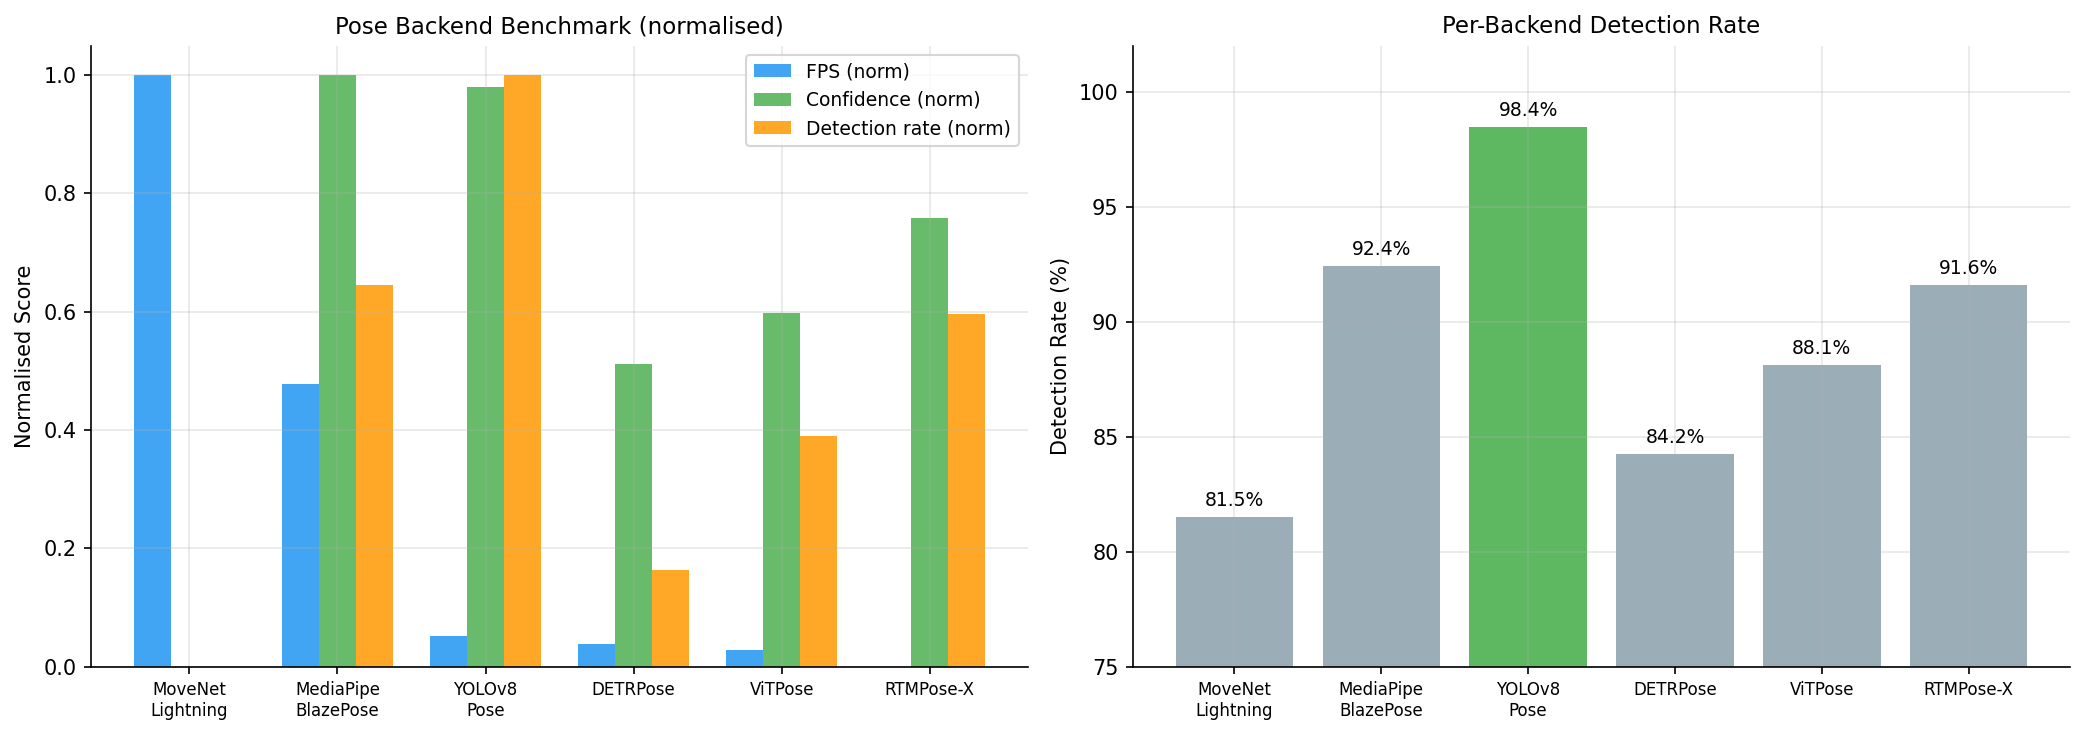
\includegraphics[width=\linewidth]{docs/figures/fig_pose_backends.png}
    \caption{\textbf{Pose backend benchmark summary.} Left: min--max normalised scores for FPS, keypoint confidence, and detection rate across all six evaluated backends. Right: raw detection rate per backend; YOLOv8-Pose (highlighted) is the only framework to exceed 98\% on the full benchmark, driven by perfect localisation on the three self-occluding exercises most critical for quality assessment.}
    \label{fig:pose_backend_chart}
\end{figure}
\begin{figure}[H]
    \centering
    \includegraphics[width=0.5\linewidth]{coco17.jpg}
    \caption{Topology of COCO 17 keypoints}
    \label{fig:coco17_keypoints}
\end{figure}

\vspace{0.5cm}
\subsection{Preprocessing Pipeline}
\label{sec:preprocessing}
\vspace{0.5cm}
Raw keypoint sequences extracted from video require several preprocessing
steps before they can serve as reliable inputs to the sequence model. The
pipeline applied in PosePulse follows six sequential stages, each targeting
a distinct source of noise or cross-dataset inconsistency.

\vspace{0.5cm}
\subsubsection{Pose Estimation and Landmark Extraction}
\vspace{0.5cm}
Skeletal keypoints are extracted from each video frame using
YOLO26-Pose~\cite{26}, the pose estimation variant of the YOLO26
architecture released by Ultralytics in 2025. YOLO26-Pose is an anchor-free,
single-stage, NMS-free detector that simultaneously localises the subject
and predicts body keypoints in a single forward pass, without requiring a
separate person-detection stage. The model outputs 17 keypoints
following the COCO format --- nose, eyes, ears, shoulders, elbows, wrists,
hips, knees, and ankles --- each accompanied by a normalised confidence
score $c_j \in [0, 1]$ indicating detection reliability. Compared to its
predecessors, YOLO26-Pose introduces Residual Log-Likelihood Estimation
(RLE) for more accurate keypoint localisation and achieves up to 43\%
faster CPU inference than YOLO11-Pose, making it well-suited for
processing large video datasets~\cite{26}. All 17 keypoints are retained
in our pipeline; face landmarks (nose, eyes, ears --- indices 0--4) are
preserved in the coordinate representation as weak postural cues encoding
head orientation relative to the torso, while joint angles are derived
exclusively from the 12 body keypoints (indices 5--16). The full sets of
angle triplets and coordinate landmarks used are listed in Tables~1
and~2 respectively.
The datasets are organised into per-exercise folders containing videos of
one of the four target activities: barbell bicep curl, shoulder press,
squat, and push-up. Each video is processed frame-by-frame: YOLO26-Pose
runs inference on every frame and returns all 17 COCO keypoints as
$(x, y)$ pixel coordinates with associated confidence scores. A bilateral
validity check is then applied: a frame is retained only if the
exercise-critical body keypoints are detected with sufficient confidence on
at least one side of the body. Frames where critical joints are absent on
both sides are discarded, as they do not contain enough structural
information to support meaningful biomechanical analysis~\cite{1}. Each valid frame contributes one row to an exercise-specific CSV file
recording the frame index, the exercise class label, the $(x, y)$
coordinates of all 17 keypoints (34 coordinate values), and the 17
associated confidence scores, yielding a raw feature matrix of shape
$(\text{valid frames},\ 51)$.
\begin{table}[h]
\centering
\begin{minipage}{0.48\textwidth}
    \centering
    \caption{Angles}
    \begin{tabular}{|l|}
    \hline
    \textbf{Landmarks} \\
    \hline
    LEFT\_HIP, LEFT\_SHOULDER, LEFT\_ELBOW \\
    \hline
    RIGHT\_HIP, RIGHT\_SHOULDER, RIGHT\_ELBOW \\
    \hline
    LEFT\_SHOULDER, LEFT\_ELBOW, LEFT\_WRIST \\
    \hline
    RIGHT\_SHOULDER, RIGHT\_ELBOW, RIGHT\_WRIST \\
    \hline
    LEFT\_SHOULDER, LEFT\_HIP, LEFT\_KNEE \\
    \hline
    RIGHT\_SHOULDER, RIGHT\_HIP, RIGHT\_KNEE \\
    \hline
    LEFT\_HIP, LEFT\_KNEE, LEFT\_ANKLE \\
    \hline
    RIGHT\_HIP, RIGHT\_KNEE, RIGHT\_ANKLE \\
    \hline
    \end{tabular}
    \label{tab:angles}
\end{minipage}
\hfill
\begin{minipage}{0.48\textwidth}
    \centering
    \caption{Coordinates}
    \begin{tabular}{|l|}
    \hline
    \textbf{Landmarks} \\
    \hline
    NOSE \\
    \hline
    LEFT\_EYE, RIGHT\_EYE \\
    \hline
    LEFT\_EAR, RIGHT\_EAR \\
    \hline
    LEFT\_SHOULDER, RIGHT\_SHOULDER \\
    \hline
    LEFT\_ELBOW, RIGHT\_ELBOW \\
    \hline
    LEFT\_WRIST, RIGHT\_WRIST \\
    \hline
    LEFT\_HIP, RIGHT\_HIP \\
    \hline
    LEFT\_KNEE, RIGHT\_KNEE \\
    \hline
    LEFT\_ANKLE, RIGHT\_ANKLE \\
    \hline
    \end{tabular}
    \label{tab:coordinates}
\end{minipage}
\end{table}

\vspace{0.5cm}
\subsubsection{Spatial Imputation of Missing Keypoints}
\vspace{0.5cm}
YOLO26-Pose assigns a confidence score to each of the 17 COCO keypoints
per frame. Joints falling below a confidence threshold of $\tau = 0.3$ ~\cite{purkrabek2025probpose}
typically caused by self-occlusion, motion blur, or partial frame
visibility --- are treated as missing and imputed using skeleton-aware
neighbour averaging: each low-confidence joint is replaced by the mean
position of its anatomically adjacent joints as defined by the COCO-17
skeleton graph in Fig ~\ref{fig:coco17_keypoints}. If no sufficiently confident skeleton neighbour exists within the COCO-17
adjacency graph, the joint falls back to the centroid of all valid joints
in the frame. This fallback is rare in practice given YOLO26-Pose's high
detection rate on single-person gym footage, but ensures no missing values
propagate to downstream feature computation.

\vspace{0.5cm}
\subsubsection{Skeleton-Based Normalisation}
\vspace{0.5cm}
Raw keypoint coordinates output by YOLO26-Pose are expressed in pixel
space and are therefore sensitive to the subject's distance from the
camera and their absolute position within the frame. Due to the varying
positions and proportions of the human body across videos, directly using
pixel coordinates as model inputs causes the same exercise performed at
different distances to produce feature vectors of very different magnitudes,
degrading classification accuracy~\cite{10, 7}. To remove these effects,
all keypoints are translated to a hip-centred coordinate system and scaled
by torso length. Let $\mathbf{h}$ denote the hip midpoint, $\mathbf{s}$
the shoulder midpoint, and $L_T$ the torso length:
\begin{equation}
\mathbf{h} = \frac{\mathbf{p}_{\text{lhip}} + \mathbf{p}_{\text{rhip}}}{2},
\qquad
\mathbf{s} = \frac{\mathbf{p}_{\text{lshoulder}} +
\mathbf{p}_{\text{rshoulder}}}{2}
\end{equation}
\begin{equation}
L_T = \|\mathbf{s} - \mathbf{h}\|_2
\end{equation}
\begin{equation}
\tilde{\mathbf{p}}_j =
\begin{cases}
\dfrac{\mathbf{p}_j - \mathbf{h}}{L_T} & \text{if } L_T > 0
\text{ and all reference joints are valid} \\[8pt]
\mathbf{p}_j & \text{otherwise}
\end{cases}
\end{equation}
where $\tilde{\mathbf{p}}_j \in \mathbb{R}^2$ is the normalised coordinate
of joint $j$~\cite{10, 7}. If any of the four reference joints ---
left/right shoulder, left/right hip --- are missing (all-zero), or if the
computed torso length is zero, the frame is returned unnormalised to avoid
division instability. This fallback affects only a negligible fraction of
frames in practice, as the shoulder and hip joints are among the most
reliably detected by YOLO26-Pose in frontal gym exercise footage. The
normalisation removes positional and scale variance by shifting each
skeleton into a body-centric coordinate system with the hip midpoint at
the origin, directly reducing spatial variability in joint coordinates
across samples of the same action class.

\vspace{0.5cm}
\subsubsection{Temporal Imputation}
\vspace{0.5cm}
Following per-frame spatial imputation, joints that flicker in and out
of confidence across consecutive frames --- a common artefact of rapid
exercise movements --- are corrected through per-joint linear interpolation
along the frame index axis. Let $t \in \{0, \ldots, T-1\}$ denote the
discrete frame index, and let $\mathcal{T}_j = \{t : c_{j,t} \geq \tau\}$
denote the set of reliably detected frames for joint $j$. The imputed
trajectory $\hat{p}_{j,d}(t)$ for coordinate dimension $d$ is defined as:
\begin{equation}
\hat{p}_{j,d}(t) =
\begin{cases}
p_{j,d}(t) & \text{if } t \in \mathcal{T}_j \\[6pt]
p_{j,d}(t_a) + \dfrac{t - t_a}{t_b - t_a}
\bigl(p_{j,d}(t_b) - p_{j,d}(t_a)\bigr)
& \text{if } t \notin \mathcal{T}_j,\ t_a \text{ and } t_b \text{ exist}
\\[6pt]
p_{j,d}(t^*) & \text{otherwise}
\end{cases}
\end{equation}
where $t_a = \max\{t' \in \mathcal{T}_j : t' \leq t\}$ and
$t_b = \min\{t' \in \mathcal{T}_j : t' \geq t\}$ are the nearest reliable
anchor frames on either side of the gap, and $t^* \in \mathcal{T}_j$ is
the nearest reliable frame when one side is absent~\cite{24}.
Specifically, for frames before the first reliable detection or after the
last reliable detection --- where a two-sided anchor pair does not exist ---
the coordinate is held constant at the nearest endpoint value, consistent
with the default behaviour of \texttt{numpy.interp}. Reliably detected
frames ($t \in \mathcal{T}_j$) are passed through unchanged, ensuring
that temporally stable joints are entirely unaffected.

\vspace{0.5cm}
\subsubsection{Biomechanical Feature Extraction}
\vspace{0.5cm}
\label{sec:vitpose}
The four preprocessing stages described in Sections~\ref{sec:preprocessing}--3.2.4
— bounding-box stabilisation, keypoint smoothing, normalisation, and occlusion
handling — constitute the proposed feature extraction pipeline. Applied to the
cleaned keypoint tensor $\mathbf{F}_k \in \mathbb{R}^{T \times 17 \times 2}$,
they produce a compact mixed biomechanical descriptor that concatenates two
complementary components. First, planar 2D joint angles are computed from fixed
anatomical triplets $(a,\,\text{vertex}\;b,\,c)$ in degrees, covering left and
right elbow, knee, hip, and shoulder joints (8 angles). Second, the normalised
$(x, y)$ coordinates of all 17 COCO keypoints are appended, contributing 34
values. The two components are concatenated to yield a descriptor
$\mathbf{v}_t \in \mathbb{R}^{42}$ per frame. This representation is fully
interpretable, requires no GPU at extraction time, and captures both joint
kinematics and skeletal geometry.

To assess whether this hand-crafted pipeline captures sufficiently discriminative
structure, it is compared against two pretrained visual encoders used as feature
extractors, replacing the angle descriptor with a higher-dimensional learned
embedding $\mathbf{F} \in \mathbb{R}^{T \times D}$.

\textbf{ViTPose-S pathway.} ViTPose~\cite{21} uses a plain Vision Transformer (ViT)
backbone pretrained with Masked Autoencoder (MAE)~\cite{he2022mae} objectives on
the MS-COCO~\cite{lin2014coco} Human Keypoint dataset, providing rich representations
of human body configuration without task-specific feature engineering. For each video
frame, YOLOv8-Pose~\cite{20} produces a cropped person region which is passed to the
frozen ViTPose-S encoder; global average pooling over the spatial token dimension
yields $\mathbf{v}_t \in \mathbb{R}^{256}$ per frame.

\textbf{ResNet pathway.} As a second reference, torchvision ResNet~\cite{he2016resnet}
models pretrained on ImageNet-1K~\cite{russakovsky2015imagenet} are used with the
classification head removed. ResNet-50 yields $\mathbf{v}_t \in \mathbb{R}^{2048}$
per frame; ResNet-18 and ResNet-34 yield 512-dimensional vectors. All ResNet
backbones are fully frozen during training.

If the proposed angle-keypoints descriptor achieves comparable performance to these
high-capacity encoders, it confirms that the preprocessing stages extract the
features most salient for exercise analysis while remaining computationally
lightweight.

\vspace{0.3cm}
\subsubsection{Temporal Windowing and Standardisation}
\vspace{0.3cm}
Exercise videos vary significantly in length ($T \in [150, 900]$ frames).
Sequence models (BiLSTM, xLSTM) require fixed input dimensions, so each
feature sequence $\mathbf{F} \in \mathbb{R}^{T \times D}$ is partitioned
into overlapping temporal windows of a configurable length $W$ with a
configurable stride $S$. The window length is chosen to capture a
sufficient number of frames to represent a meaningful movement unit ---
typically one complete phase transition such as the descent of a squat ---
while the stride controls the degree of overlap and the number of windows
generated per video. Each window is assigned the exercise label of its
first frame; since each video contains only one exercise type, this label
is constant across all windows from the same video~\cite{1}.

Before training, all $D$ features are standardised to zero mean and unit
variance using statistics computed from the training set:
$\mathbf{X}_{\text{std}} = (\mathbf{X} - \boldsymbol{\mu}) /
\boldsymbol{\sigma}$. Standardisation improves gradient flow and allows
BiLSTM and xLSTM to focus on relative magnitudes rather than absolute
scales. Parameters $(\boldsymbol{\mu}, \boldsymbol{\sigma})$ are computed
once from the training set and applied identically to validation and test
sets to prevent data leakage.

\vspace{0.4cm}
\subsection{Model Architectures}
PosePulse trains two sequence classification models: a Bidirectional LSTM--CNN
hybrid and an xLSTM following the \texttt{xLSTM[7:1]} configuration of
Beck et al.~\cite{4}. Both models receive the same standardised input
and are trained with the AdamW optimiser.

\vspace{0.4cm}
\begin{figure}[H]
    \centering
    \includegraphics[width=\linewidth, height = 8cm]{bilstm_final .png}
    \caption{The BiLSTM processes 30-frame windows bidirectionally, the output is reshaped and refined by three Conv2D layers with
ReLU activations, and a Softmax head predicts one of four
exercise classes.}
    \label{fig:bilstm_arch}
\end{figure}

\subsubsection{Bidirectional LSTM-CNN}
\vspace{0.3cm}
The input tensor $\mathbf{F} \in \mathbb{R}^{N \times 30 \times 256}$
is passed through a Bidirectional LSTM layer with 64 hidden units per
direction. At each timestep $t$, the forward and backward cells compute:
\begin{equation}
\overrightarrow{\mathbf{h}}_t = \text{LSTM}_{\text{fwd}}
(\mathbf{f}_t,\ \overrightarrow{\mathbf{h}}_{t-1}), \qquad
\overleftarrow{\mathbf{h}}_t = \text{LSTM}_{\text{bwd}}
(\mathbf{f}_t,\ \overleftarrow{\mathbf{h}}_{t+1})
\end{equation}
The concatenated hidden state $\mathbf{h}_t =
[\overrightarrow{\mathbf{h}}_t;\ \overleftarrow{\mathbf{h}}_t] \in
\mathbb{R}^{8}$ captures bidirectional temporal context at each frame,
yielding an output sequence $\mathbf{H} \in \mathbb{R}^{30 \times 8}$.
This is reshaped to $(N,\ 1,\ 30,\ 8)$ --- a single-channel
two-dimensional map with time along one spatial axis and hidden
features along the other --- to serve as input to the convolutional
stage.
\textbf{Convolutional Refinement.}
Three successive Conv2D layers with ReLU activations extract local
patterns across the time--feature map:
\begin{equation}
\mathbf{Z}^{(l)} = \text{ReLU}\!\left(
\mathbf{W}^{(l)} * \mathbf{Z}^{(l-1)} + \mathbf{b}^{(l)}
\right), \quad l \in \{1, 2, 3\}
\end{equation}
The three layers use 128, 256, and 64 filters respectively, each
operating on the $(30 \times 8)$ spatial map. The first two layers
progressively expand the feature representation; the third compresses
it back. A final Conv2D layer reduces the channel dimension to 1, and
the resulting feature map is flattened and passed through a linear
classification head with Softmax output over the four exercise classes
(squat, push-up, shoulder press, bicep curl).

\vspace{0.3cm}
\subsubsection{xLSTM}
\vspace{0.3cm}
The xLSTM model follows the \texttt{xLSTM[7:1]} block configuration
identified as best-performing among LSTM-class models in Beck et
al.~\cite{4}, which achieved the lowest validation perplexity among
all LSTM, SSM, RNN, and linear Transformer baselines on the SlimPajama
benchmark. Although this result was obtained in a language modelling
context, the architectural properties that drive the gain --- exponential
gating, high-capacity matrix memory, and residual block stacking --- are
general sequence modelling advantages that transfer to biomechanical
time-series classification, where capturing long-range dependencies
across a 30-frame or 60-frame movement windows is equally critical. The notation
\texttt{xLSTM[7:1]} denotes 7 mLSTM blocks for every 1 sLSTM block,
giving 8 residually stacked blocks in total~\cite{4}.
\begin{figure}[H]
    \centering
    
\includegraphics[width = \linewidth, height = 8cm]{xlstm_final.png}
    \caption{xLSTM[7:1] architecture for exercise classification.
Extracted features are passed through 8 residually
stacked xLSTM blocks (7 mLSTM + 1 sLSTM) with LayerNorm and skip
connections. The output sequence is mean-pooled over the time
dimension, passed through dropout, and projected via a linear
Softmax head to four exercise classes.}
    \label{fig:xlstm_arch}
\end{figure}
\textbf{sLSTM (scalar LSTM).} The sLSTM cell introduces exponential
gating with a scalar memory and a scalar update rule, and adds a new
memory mixing technique via hidden-hidden recurrent connections.
For input $\mathbf{x}_t$ and previous hidden state $\mathbf{h}_{t-1}$,
the cell computes input gate $i_t = \exp(\tilde{i}_t)$, forget gate
$f_t = \exp(\tilde{f}_t)$, and output gate $o_t = \sigma(\tilde{o}_t)$
with stabilised normaliser $n_t = f_t n_{t-1} + i_t$:
\begin{equation}
c_t = f_t c_{t-1} + i_t z_t, \qquad
h_t = o_t \cdot \psi\!\left(\frac{c_t}{n_t}\right)
\end{equation}
where $z_t = \tanh(\mathbf{W}_z \mathbf{x}_t + \mathbf{R}_z
\mathbf{h}_{t-1})$ is the cell input and $\psi$ is a stabilisation
function. Memory mixing via the recurrent matrix $\mathbf{R}_z$ allows
the sLSTM to solve state-tracking problems that SSMs and standard
Transformers cannot~\cite{4}.
\textbf{mLSTM (matrix LSTM).} The mLSTM replaces the scalar memory
with a matrix memory cell state $\mathbf{C}_t \in \mathbb{R}^{d \times
d}$ updated via a covariance rule, making it fully parallelisable by
abandoning hidden-hidden recurrent connections. Queries, keys, and
values are projected from the input: $\mathbf{q}_t = \mathbf{W}_q
\mathbf{x}_t$, $\mathbf{k}_t = \mathbf{W}_k \mathbf{x}_t / \sqrt{d}$,
$\mathbf{v}_t = \mathbf{W}_v \mathbf{x}_t$. Memory and normaliser are
updated as:
\begin{equation}
\mathbf{C}_t = f_t \mathbf{C}_{t-1} + i_t \mathbf{v}_t \mathbf{k}_t^\top,
\qquad
\mathbf{n}_t = f_t \mathbf{n}_{t-1} + i_t \mathbf{k}_t
\end{equation}
The hidden state is retrieved as:
\begin{equation}
\tilde{\mathbf{h}}_t = \frac{\mathbf{C}_t \mathbf{q}_t}
{\max(|\mathbf{n}_t^\top \mathbf{q}_t|,\ 1)}, \qquad
\mathbf{h}_t = \mathbf{o}_t \odot \tilde{\mathbf{h}}_t
\end{equation}
where $f_t$ and $i_t$ use exponential gating with a running maximum
stabiliser $m_t = \max(\tilde{f}_t + m_{t-1},\ \tilde{i}_t)$ to
prevent numerical overflow~\cite{4}.
\textbf{xLSTM Block Stack.} Each mLSTM block uses a pre up-projection
residual design: the input is projected to a higher-dimensional space,
processed by the mLSTM, and projected back, wrapped with a learnable
skip connection, a causal convolution, and an output gate. Each sLSTM
block uses a post up-projection design followed by a gated MLP,
consistent with Transformer residual blocks. All 8 blocks apply
LayerNorm and residual connections, with hidden dimension $d = 256$.
The output sequence is mean-pooled over the 30-frame or 60-frame time dimension,
passed through a dropout layer, and projected via a linear Softmax
head to four exercise classes (squat, push-up, shoulder press, bicep
curl).

\vspace{0.4cm}
\subsubsection{Multi-Task xLSTM for Quality Assessment and Coaching Feedback}
\vspace{0.3cm}
Building on the EgoExo-Fitness dataset introduced in Section~2.2,
PosePulse extends the single-task xLSTM into a \emph{branched
multi-task} model. Exercise quality is predicted by a learned
regression head; coaching guidance and corrective comments are both
delivered by zero-parameter retrieval lookups and require no
additional learned components. The full pipeline is illustrated in
Figure~\ref{fig:egoexo_arch}.

\begin{figure}[H]
    \centering
    \includegraphics[width=0.85\linewidth]{xlstm-multitask-arch.png}
    \caption{\textbf{Branched multi-task xLSTM architecture for EgoExo-Fitness.}
    Pre-extracted CLIP ViT-B/32 frame embeddings (512-d) are projected to 256-d
    and processed by a shared eight-block all-mLSTM encoder
    (\texttt{block\_pattern = mmmmmmmm}).
    Attention pooling produces a clip embedding $\mathbf{e} \in \mathbb{R}^{256}$,
    which is split into two task-specialised branches: Branch~A
    (LN\,\textrightarrow\,Linear\,\textrightarrow\,GELU) feeds the classification
    head exclusively, and Branch~B feeds the quality head exclusively, preventing
    gradient interference between tasks. Coaching feedback is retrieval-based and
    parameter-free: the predicted class $\hat{y}$ indexes a guidance lookup table,
    while the pair $(\hat{y},\,\mathrm{bucket}(\hat{q}))$ indexes a corrective
    comment table with equal-frequency quality bins.}
    \label{fig:egoexo_arch}
\end{figure}

\textbf{Feature Extraction.}
The EgoExo-Fitness clips are represented by pre-extracted CLIP
ViT-B/32 frame features~\cite{21} at 512 dimensions. A learned linear
projection maps each frame to 256-d, producing the tensor
$\mathbf{F} \in \mathbb{R}^{T \times 256}$ consumed by the
xLSTM stack.

\textbf{Shared Encoder.}
The encoder is an eight-block \textbf{all-mLSTM} stack
(\texttt{block\_pattern = mmmmmmmm})~\cite{4}, trading the sLSTM
block's state-tracking capability for full parallelism — the
short, fixed-length clips in EgoExo-Fitness do not require
the sequential state updates that sLSTM provides, and the
all-mLSTM variant trains faster on the same hardware. The
encoder yields the output sequence
$\mathbf{H} \in \mathbb{R}^{T \times 256}$. The sequence
is then summarised by a learned attention pooling layer:
\begin{equation}
    \alpha_t = \frac{\exp(\mathbf{w}^{\top}\mathbf{h}_t)}
                    {\sum_{t'}\exp(\mathbf{w}^{\top}\mathbf{h}_{t'})},
    \qquad
    \mathbf{e} = \sum_{t}\alpha_t\,\mathbf{h}_t \;\in\; \mathbb{R}^{256},
\end{equation}
where $\mathbf{w} \in \mathbb{R}^{256}$ is a learnable scoring vector.
Attention pooling allows the model to suppress uninformative frames and
concentrate on the most diagnostically relevant moments in the clip.

\textbf{Branched Multi-Task Fusion.}
The clip embedding $\mathbf{e}$ feeds two parallel branches, each
consisting of LayerNorm, a linear projection
$\mathbb{R}^{256} \!\rightarrow\! \mathbb{R}^{128}$, and a GELU
activation, with independent weights:
\begin{equation}
\mathbf{a} = \mathrm{GELU}(\mathrm{Linear}_A(\mathrm{LN}_A(\mathbf{e}))),
\qquad
\mathbf{b} = \mathrm{GELU}(\mathrm{Linear}_B(\mathrm{LN}_B(\mathbf{e}))).
\end{equation}
Branch A is the sole pathway to the classification head; Branch B is
the sole pathway to the quality head. Routing gradients exclusively
through their respective branches prevents interference between the
two objectives during training.

\textbf{Task Heads.}
The classification head projects $\mathbf{a} \in \mathbb{R}^{128}$
to 12 logits via a linear layer followed by softmax, trained with
cross-entropy loss ($\mathcal{L}_{\mathrm{cls}}$). The quality head
projects $\mathbf{b} \in \mathbb{R}^{128}$ to a scalar through a
linear layer followed by sigmoid, producing
$\hat{q} \in [0,1]$, trained with smooth-$L_1$ loss
($\mathcal{L}_{\mathrm{quality}}$).

\textbf{Encoder Initialisation and Partial Fine-Tuning.}
The xLSTM encoder weights are initialised from the classification
checkpoint trained on the Riccio dataset, then frozen. Only the last
two encoder layers are released for gradient updates. This strategy
prevents catastrophic forgetting of the classification representations
while allowing the encoder to adapt to the quality-discriminative
signal in EgoExo-Fitness — particularly important given the relatively
small corpus of 1{,}525 annotated clips.

\textbf{Multi-Task Loss Scheduling via DWA.}
Naively summing the classification and quality losses with fixed
weights risks one task dominating gradient updates. To avoid this,
task-loss weights are adapted automatically at each epoch using
\textbf{Dynamic Weight Averaging (DWA)}~\cite{deepmtl2r}. Let
$\ell_k(t)$ denote the loss of task $k$ at epoch $t$ and $K$ the
number of tasks. The weight assigned to task $k$ is:
\begin{equation}
    w_k(t) = \frac{K \cdot \exp\!\left(r_k(t-1)/T\right)}
                  {\sum_{i=1}^{K}\exp\!\left(r_i(t-1)/T\right)},
    \qquad
    r_k(t) = \frac{\ell_k(t)}{\ell_k(t-1)},
\end{equation}
where $r_k(t)$ is the relative rate of loss change for task $k$ and
$T$ is a temperature controlling the sharpness of the weight
distribution. Tasks whose loss decreases slowly receive a larger
weight, directing gradient capacity toward under-optimised objectives
without manual tuning. The total loss at each training step is:
\begin{equation}
    \mathcal{L}(t) = w_{\mathrm{cls}}(t)\,\mathcal{L}_{\mathrm{cls}}
    + w_{\mathrm{quality}}(t)\,\mathcal{L}_{\mathrm{quality}},
\end{equation}
with a DWA history window of 25 epochs and temperature $T{=}2.0$ to
prevent the distribution from collapsing to a single task. Balanced
class weights are additionally applied to $\mathcal{L}_{\mathrm{cls}}$
to correct for the unequal exercise-class distribution in
EgoExo-Fitness.

\textbf{Coaching Feedback via Retrieval.}
As established in Section~2.2, the \texttt{action\_guidance} field is
class-deterministic, motivating a zero-parameter lookup
$\mathcal{G}: \hat{y} \mapsto \text{text}$ populated from the
training split. Coaching comments are retrieved from a second
lookup table indexed jointly by the predicted class $\hat{y}$ and a
quality bucket $\mathrm{bucket}(\hat{q})$, where the training
quality distribution is discretised into three equal-frequency buckets
(low\,/\,mid\,/\,high). Each cell $(c,\,b)$ is populated with the
training comment whose normalised quality is closest to the bucket
centre; cross-class fallback is forbidden by design. Together, the
two lookup tables deliver four coaching outputs — exercise label,
quality score, guidance, and corrective comment — at $O(1)$
retrieval latency with no additional learned parameters.

\vspace{0.4cm}
\section{Experiments and Results}
\label{sec:experiments}
\subsection{Training Configuration}
Both classification models are trained under shared data and evaluation
protocols. The BiLSTM--CNN additionally uses a single shared optimiser,
schedule, and window configuration across all three feature conditions
(Table~\ref{tab:bilstm_hparams}). The xLSTM[7:1] requires per-condition
tuning of the temporal window length and optimiser settings
(Table~\ref{tab:xlstm_hparams}): under the ViTPose-S feature condition,
the 30-frame window inherited from the BiLSTM--CNN protocol produced
noticeably weaker results than expected, with the xLSTM[7:1] failing to
match the BiLSTM--CNN's macro F1 despite its larger capacity. This
empirical observation motivated an expanded 60-frame window for the
hand-crafted and ResNet-50 conditions, accompanied by a smaller
learning rate, lower minimum learning rate, stronger weight decay, and
longer training horizon to keep optimisation stable under the longer
effective context.  The pipeline-shared protocol common to all six
(model, feature) combinations is summarised in
Table~\ref{tab:conditions}.

\begin{table}[H]
\centering
\caption{Feature extraction conditions. All other pipeline stages
are identical across conditions.}
\label{tab:conditions}
\small
\renewcommand{\arraystretch}{1.15}
\begin{tabular}{|l|l|c|l|}
\hline
\textbf{Condition} & \textbf{Feature source} & \textbf{Dim} &
\textbf{Pretrained on} \\
\hline
Hand-crafted & 8 joint angles + 34 COCO coordinates & 42 &
  COCO (YOLO26-Pose only) \\
ResNet-50    & Global avg-pool of ResNet-50 person crop & 2{,}048 &
  ImageNet-1k \\
ViTPose-S    & Token-pooled ViTPose-S person crop & 256 &
  COCO Keypoint~\cite{xu2022vitpose} \\
\hline
\end{tabular}
\end{table}

\begin{table}[H]
\centering
\caption{BiLSTM--CNN best hyperparameters. The same configuration is used
across all three feature conditions.}
\label{tab:bilstm_hparams}
\small
\renewcommand{\arraystretch}{1.15}
\begin{tabular}{|l|l|}
\hline
\textbf{Setting} & \textbf{Value} \\
\hline
Hidden dimension      & 64 per direction (128 concat.) \\
Depth                 & 1 BiLSTM + 4 Conv2D layers (kernels 128, 256, 64, 1; all $3{\times}3$) \\
Temporal pooling      & flattened conv feature map \\
Dropout               & $0.3$ \\
Window length         & 30 frames \\
Learning rate         & $3 \times 10^{-4}$ $\rightarrow$ $\eta_{\min} = 3 \times 10^{-6}$ (cosine) \\
Weight decay $\lambda$& $10^{-4}$ \\
Batch size            & $64$ \\
Total epochs          & $35$ \\
Total parameters      & $\sim$3.0\,M \\
\hline
\end{tabular}
\end{table}

\begin{table}[H]
\centering
\caption{xLSTM[7:1] best hyperparameters split by feature condition.
Hand-crafted and ResNet-50 use a 60-frame window with a smaller
learning rate, lower $\eta_{\min}$, stronger weight decay, and a
longer training horizon, because the 30-frame configuration that
suffices for the BiLSTM--CNN was empirically unstable for the
matrix-memory mLSTM stack on those two representations. ViTPose-S
retains the 30-frame configuration.}
\label{tab:xlstm_hparams}
\small
\renewcommand{\arraystretch}{1.15}
\begin{tabular}{|l|l|l|}
\hline
\textbf{Setting} & \textbf{ViTPose-S} & \textbf{Hand-crafted \& ResNet-50} \\
\hline
Block pattern        & \texttt{mmmmmmms} (7 mLSTM + 1 sLSTM)
                     & \texttt{mmmmmmms} (7 mLSTM + 1 sLSTM) \\
Hidden dimension     & 256 (residual stream) & 256 (residual stream) \\
Attention heads      & 4 (per mLSTM block)   & 4 (per mLSTM block)   \\
Conv kernel          & causal Conv1D, kernel 4 & causal Conv1D, kernel 4 \\
Projection factor    & $4/3$                 & $4/3$                 \\
Temporal pooling     & mean over time         & mean over time         \\
Window length        & 30 frames              & \textbf{60 frames}     \\
Dropout              & $0.15$                 & \textbf{$0.25$}        \\
Learning rate        & $3 \times 10^{-4}$     & \textbf{$1 \times 10^{-4}$} \\
Min learning rate    & $3 \times 10^{-6}$     & \textbf{$1 \times 10^{-6}$} \\
Weight decay         & $1 \times 10^{-4}$     & \textbf{$1 \times 10^{-3}$} \\
Batch size           & $64$                   & \textbf{$32$}          \\
Total epochs         & $35$                   & \textbf{$10, 15$}          \\
Total parameters     & $\sim$5.2\,M           & $\sim$5.2\,M           \\
\hline
\end{tabular}
\end{table}

\begin{figure}[H]
    \centering
    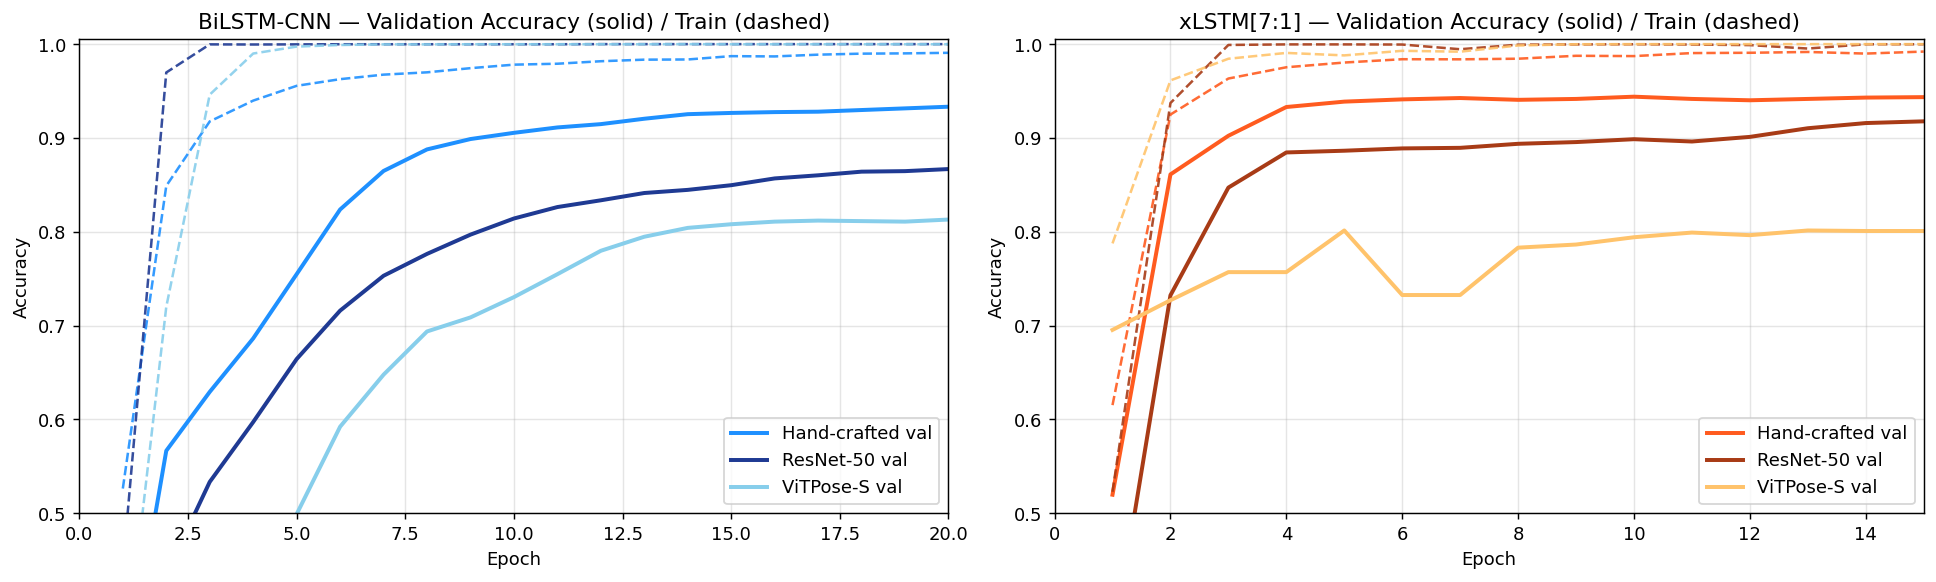
\includegraphics[width=\linewidth]{docs/figures/fig_training_curves.png}
    \caption{\textbf{Validation and training accuracy curves for all six (model, feature) conditions.} Solid lines show validation accuracy; dashed lines show training accuracy. Left panel: BiLSTM-CNN across three feature conditions. Right panel: xLSTM[7:1]. The wider train--val gap under ViTPose-S reflects the lower representational utility of pose-transformer embeddings for this task, while hand-crafted and ResNet-50 features converge to higher validation accuracy.}
    \label{fig:training_curves}
\end{figure}

\begin{table}[H]
\centering
\caption{Per-class test-set performance (F1, recall, precision, AUC)
for all six (feature, model) combinations. Best per-condition macro
value is bolded; best overall combination across the table is starred
in Table~\ref{tab:macro_summary}.}
\label{tab:perclass_results}
\scriptsize
\renewcommand{\arraystretch}{1.08}
\setlength{\tabcolsep}{3pt}
\begin{tabular}{ll|cccc|r||cccc|r}
\hline
& & \multicolumn{5}{c||}{\textbf{BiLSTM-CNN}}
  & \multicolumn{5}{c}{\textbf{xLSTM[7:1]}} \\
\textbf{Cond.} & \textbf{Class}
  & Pre & Rec & F1 & AUC & Sup
  & Pre & Rec & F1 & AUC & Sup \\
\hline
\multirow{7}{*}{\rotatebox{90}{Hand-crafted}}
  & Bicep curl     & 0.933 & 0.853 & 0.891 & 0.960 & 490
                   & 0.874 & 0.855 & 0.864 & 0.981 & 447 \\
  & Push-up        & 0.835 & 0.992 & 0.907 & 0.991 & 481
                   & 0.822 & 0.959 & 0.885 & 0.987 & 437 \\
  & Shoulder press & 0.967 & 0.886 & 0.925 & 0.976 & 632
                   & 0.969 & 0.864 & 0.914 & 0.988 & 588 \\
  & Squat          & 0.918 & 0.926 & 0.922 & 0.986 & 606
                   & 0.876 & 0.877 & 0.876 & 0.982 & 562 \\
\cline{2-12}
  & Accuracy       & \multicolumn{3}{c}{}  & \textbf{0.913} & 2{,}209
                   & \multicolumn{3}{c}{}  & \textbf{0.886}          & 2{,}034 \\
  & Macro avg      & 0.913 & 0.914 & 0.911 & 0.978 & 2{,}209
                   & 0.885 & 0.889 & 0.885 & 0.984 & 2{,}034 \\
  & Weighted avg   & 0.918 & 0.913 & 0.913 & 0.978 & 2{,}209
                   & 0.886 & 0.886 & 0.884 & 0.984 & 2{,}034 \\
\hline
\multirow{7}{*}{\rotatebox{90}{ResNet-50}}
  & Bicep curl     & 0.758 & 0.656 & 0.703 & 0.872 & 392
                   & 0.897 & 0.774 & 0.831 & 0.929 & 349 \\
  & Push-up        & 0.962 & 1.000 & 0.981 & 1.000 & 276
                   & 0.967 & 1.000 & 0.983 & 1.000 & 236 \\
  & Shoulder press & 0.878 & 0.958 & 0.916 & 0.989 & 472
                   & 0.898 & 0.991 & 0.942 & 0.984 & 428 \\
  & Squat          & 0.838 & 0.836 & 0.837 & 0.954 & 538
                   & 0.931 & 0.923 & 0.927 & 0.985 & 494 \\
\cline{2-12}
  & Accuracy       & \multicolumn{3}{c}{}  & \textbf{0.855} & 1{,}678
                   & \multicolumn{3}{c}{}  & \textbf{0.920} & 1{,}507 \\
  & Macro avg      & 0.859 & 0.862 & 0.859 & 0.954 & 1{,}678
                   & 0.923 & 0.922 & 0.921 & 0.974 & 1{,}507 \\
  & Weighted avg   & 0.851 & 0.855 & 0.852 & 0.952 & 1{,}678
                   & 0.919 & 0.920 & 0.918 & 0.974 & 1{,}507 \\
\hline
\multirow{7}{*}{\rotatebox{90}{ViTPose-S}}
  & Bicep curl     & 0.588 & 0.671 & 0.627 & 0.886 & 392
                   & 0.701 & 0.653 & 0.676 & 0.936 & 392 \\
  & Push-up        & 1.000 & 1.000 & 1.000 & 1.000 & 276
                   & 0.985 & 0.975 & 0.980 & 0.998 & 276 \\
  & Shoulder press & 0.901 & 0.833 & 0.866 & 0.907 & 472
                   & 0.875 & 0.828 & 0.851 & 0.968 & 472 \\
  & Squat          & 0.711 & 0.686 & 0.698 & 0.883 & 538
                   & 0.676 & 0.745 & 0.709 & 0.913 & 538 \\
\cline{2-12}
  & Accuracy       & \multicolumn{3}{c}{}  & \textbf{0.775} & 1{,}678
                   & \multicolumn{3}{c}{}  & \textbf{0.785} & 1{,}678 \\
  & Macro avg      & 0.800 & 0.797 & 0.798 & 0.919 & 1{,}678
                   & 0.809 & 0.800 & 0.804 & 0.954 & 1{,}678 \\
  & Weighted avg   & 0.783 & 0.775 & 0.778 & 0.910 & 1{,}678
                   & 0.789 & 0.785 & 0.786 & 0.948 & 1{,}678 \\
\hline
\end{tabular}
\end{table}

\vspace{0.3cm}
Three findings stand out from Table~\ref{tab:perclass_results} and
Fig.~\ref{fig:macro_comparison}.
First, the hand-crafted 42-d descriptor achieves the strongest
overall results under BiLSTM-CNN (accuracy 91.3\%, macro
F1\,=\,0.911), confirming that the four preprocessing stages are
highly discriminative without a GPU or pretrained backbone.
Second, xLSTM[7:1] substantially outperforms BiLSTM-CNN under
ResNet-50 (macro F1\,=\,0.921 vs.\ 0.859), indicating its
matrix-memory is better suited to richer 2048-d appearance sequences.
Third, ViTPose-S is the weakest condition for both models
(accuracy 77.5--78.5\%), likely because pose-transformer embeddings
encode heatmap distributions rather than the joint-angle trajectories
most informative for exercise discrimination.
Push-up is the most easily separated class across conditions, while
bicep curl is consistently the most challenging, consistent with the
self-occlusion identified in Section~3.1.
Were classification the sole objective, xLSTM[7:1] with ResNet-50
(92.0\%, macro F1\,=\,0.921) would be preferred; the hand-crafted
descriptor remains a lightweight alternative within 0.7 percentage
points while requiring no GPU at extraction time.

\begin{figure}[H]
    \centering
    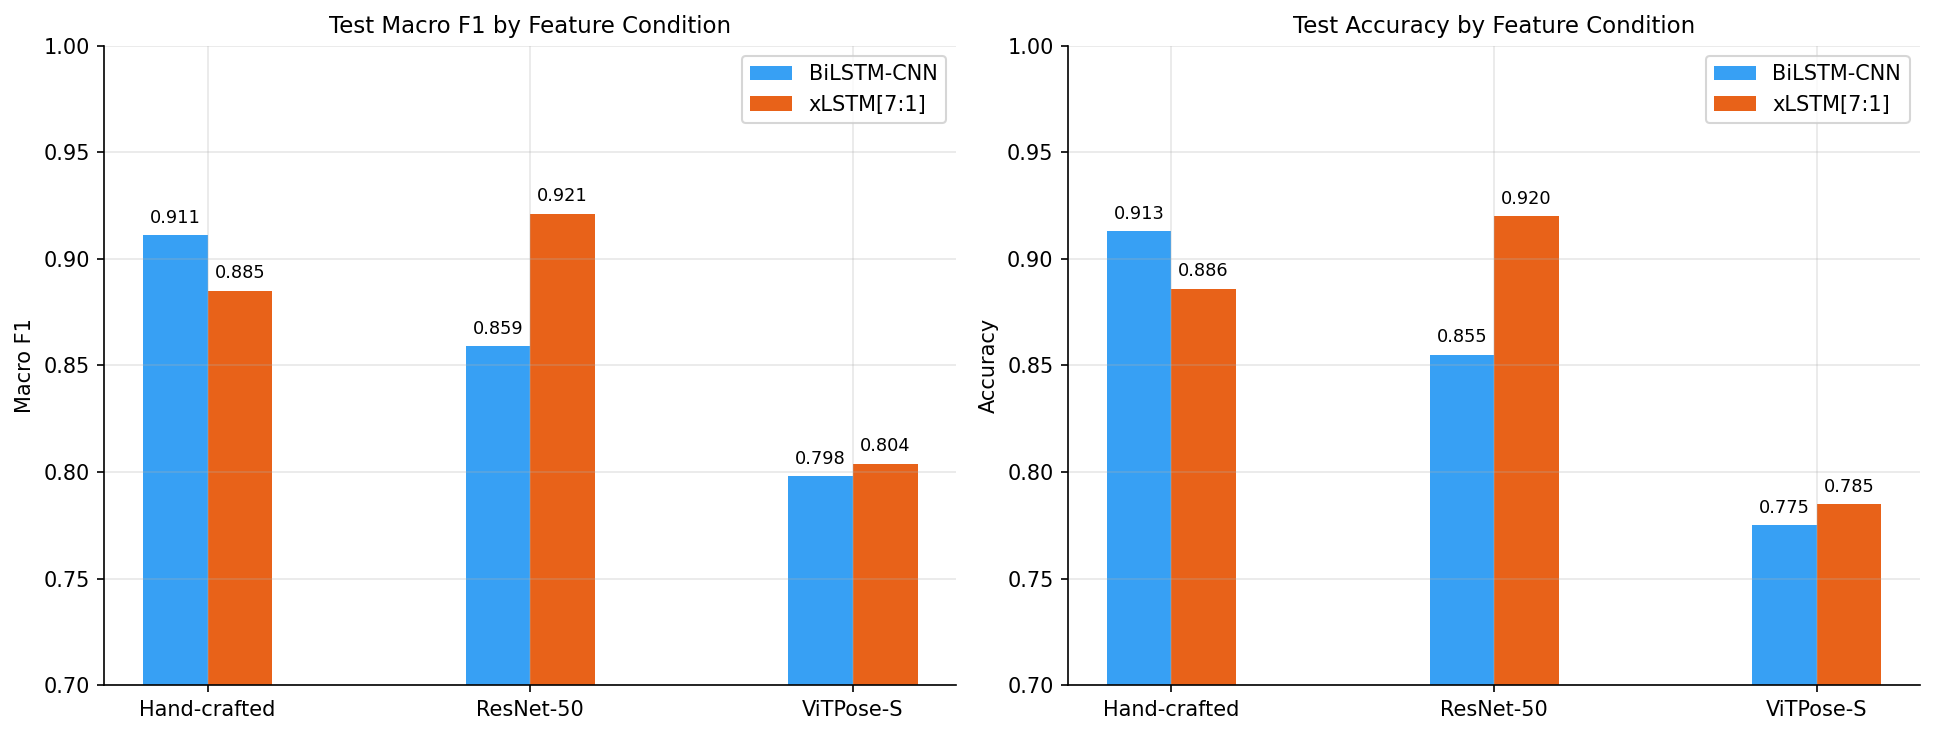
\includegraphics[width=\linewidth]{docs/figures/fig_macro_comparison.png}
    \caption{\textbf{Macro F1 and accuracy comparison across all six (model, feature) conditions.} xLSTM[7:1] achieves the highest overall scores under ResNet-50 features (macro F1\,=\,0.921, accuracy 92.0\%), while BiLSTM-CNN leads under hand-crafted features (macro F1\,=\,0.911, accuracy 91.3\%). ViTPose-S is the weakest condition for both models.}
    \label{fig:macro_comparison}
\end{figure}

\subsection{Multi-Task xLSTM Training on EgoExo-Fitness}
\label{sec:multitask_config}

The multi-task xLSTM is trained on pre-extracted CLIP ViT-B/32 features
drawn from all available camera views in EgoExo-Fitness, treating each
(clip, view) pair as an independent training sample to maximise data
coverage. Several configuration decisions differ deliberately from the
classification-only setting and are motivated by the distinct properties
of the EgoExo-Fitness corpus.

\textbf{All-mLSTM block pattern.} The classification models use the
\texttt{mmmmmmms} pattern (seven mLSTM + one sLSTM block). For the
multi-task setting the sLSTM block is replaced by a further mLSTM
block, yielding the pure all-mLSTM pattern \texttt{mmmmmmmm}. The
60-frame EgoExo clips are shorter and more temporally uniform than the
long gym sequences used for classification; they do not benefit from
the sLSTM's state-tracking capability, and the all-mLSTM variant is
fully parallelisable, reducing wall-clock training time on the
available T4 GPU.

\textbf{Longer context window.} The window is extended from 30 to 60
frames with a stride of 30 (50\% overlap). A 60-frame window covers
two full seconds at the EgoExo frame rate, spanning a complete
repetition of most exercises and thereby giving the quality regression
head access to the full movement arc rather than a single phase
transition.

\textbf{Partial fine-tuning of a frozen backbone.} The xLSTM encoder
weights pretrained on the classification task are frozen and only the
last two encoder layers are released for gradient updates. This
strategy prevents catastrophic forgetting of the classification
representations while still allowing the encoder to adapt its final
layers to the quality-discriminative signal present in EgoExo-Fitness,
which is particularly important given the relatively small size of the
annotated corpus (1,525 clips).

\textbf{Multi-task loss scheduling via DWA.}
Naively summing the classification and quality losses with fixed
weights risks one task dominating gradient updates throughout training.
To avoid this, task-loss weights are adapted automatically at each
epoch using \textbf{Dynamic Weight Averaging (DWA)}, following the
multi-task loss scheduling methodology of
\textbf{DeepMTL2R}~\cite{deepmtl2r}. Let $\ell_k(t)$ denote the loss
of task $k$ at epoch $t$ and $K$ the number of tasks. The weight
assigned to task $k$ is:

\begin{equation}
    w_k(t) = \frac{K \cdot \exp\!\left(r_k(t-1)/T\right)}
                  {\sum_{i=1}^{K}\exp\!\left(r_i(t-1)/T\right)},
    \qquad
    r_k(t) = \frac{\ell_k(t)}{\ell_k(t-1)}
\end{equation}

where $r_k(t)$ is the relative rate of loss change for task $k$ and
$T$ is a temperature that controls the sharpness of the distribution.
Tasks whose loss decreases slowly (high $r_k$) receive a larger
weight, directing gradient capacity toward under-optimised objectives
without manual tuning. The total loss at each training step is:

\begin{equation}
    \mathcal{L}(t) \;=\;
    w_{\mathrm{cls}}(t)\,\mathcal{L}_{\mathrm{cls}}
    \;+\;
    w_{\mathrm{quality}}(t)\,\mathcal{L}_{\mathrm{quality}}
\end{equation}

with $\mathcal{L}_{\mathrm{cls}}$ the cross-entropy classification
loss and $\mathcal{L}_{\mathrm{quality}}$ the smooth-$L_1$ quality
regression loss. A DWA history window of 25 epochs smooths the
loss-rate signal before computing weights, and a temperature of
$T{=}2.0$ prevents the distribution from collapsing to a single task.
Balanced class weights are additionally applied to
$\mathcal{L}_{\mathrm{cls}}$ to correct for the unequal
exercise-class distribution in EgoExo-Fitness.

\textbf{Comment quality discretisation.} Coaching comments are
discretised into three equal-frequency quality buckets (low / mid /
high) derived from the training quality distribution, providing the
comment retrieval head with a coarser but more robustly estimated
supervision signal than a direct continuous target.

The full hyperparameter configuration is given in
Table~\ref{tab:multitask_hparams}.

\begin{table}[H]
\centering
\caption{Multi-task xLSTM best hyperparameters for the EgoExo-Fitness
training run. A single configuration is used across all camera views.}
\label{tab:multitask_hparams}
\footnotesize
\renewcommand{\arraystretch}{1.05}
\begin{tabular}{|l|l|}
\hline
\textbf{Setting} & \textbf{Value} \\
\hline
Block pattern          & \texttt{mmmmmmmm} (8 mLSTM, all-mLSTM) \\
Hidden dimension       & 256 (residual stream) \\
Attention heads        & 4 (per mLSTM block) \\
Conv kernel / proj.\ factor & causal Conv1D kernel 4 / $4/3$ \\
Multi-view fusion dim  & 128 \\
Temporal pooling       & attention pooling \\
Window length / stride & 60 frames / 30 frames \\
Max frames / subsample stride & 300 / 3 \\
Dropout                & $0.15$ \\
Backbone               & frozen; last 2 layers unfrozen \\
\hline
Learning rate          & $3 \times 10^{-4}$ $\rightarrow$ $\eta_{\min} = 3 \times 10^{-6}$ (cosine) \\
Warmup fraction        & 0.1 \\
Weight decay $\lambda$ & $10^{-4}$ \\
Gradient clip          & 1.0 \\
Batch size             & 32 \\
Total epochs           & 50 \\
\hline
MTL method             & Dynamic Weight Averaging (DWA) \\
DWA history window     & 25 epochs \\
DWA temperature $T$    & 2.0 \\
Error weight           & 0.0 \\
Balanced class weights & yes \\
Comment quality buckets & 3 (equal-frequency) \\
\hline
Total parameters       & $\sim$5.2\,M \\
\hline
\end{tabular}
\end{table}

\begin{figure}[H]
  \centering
  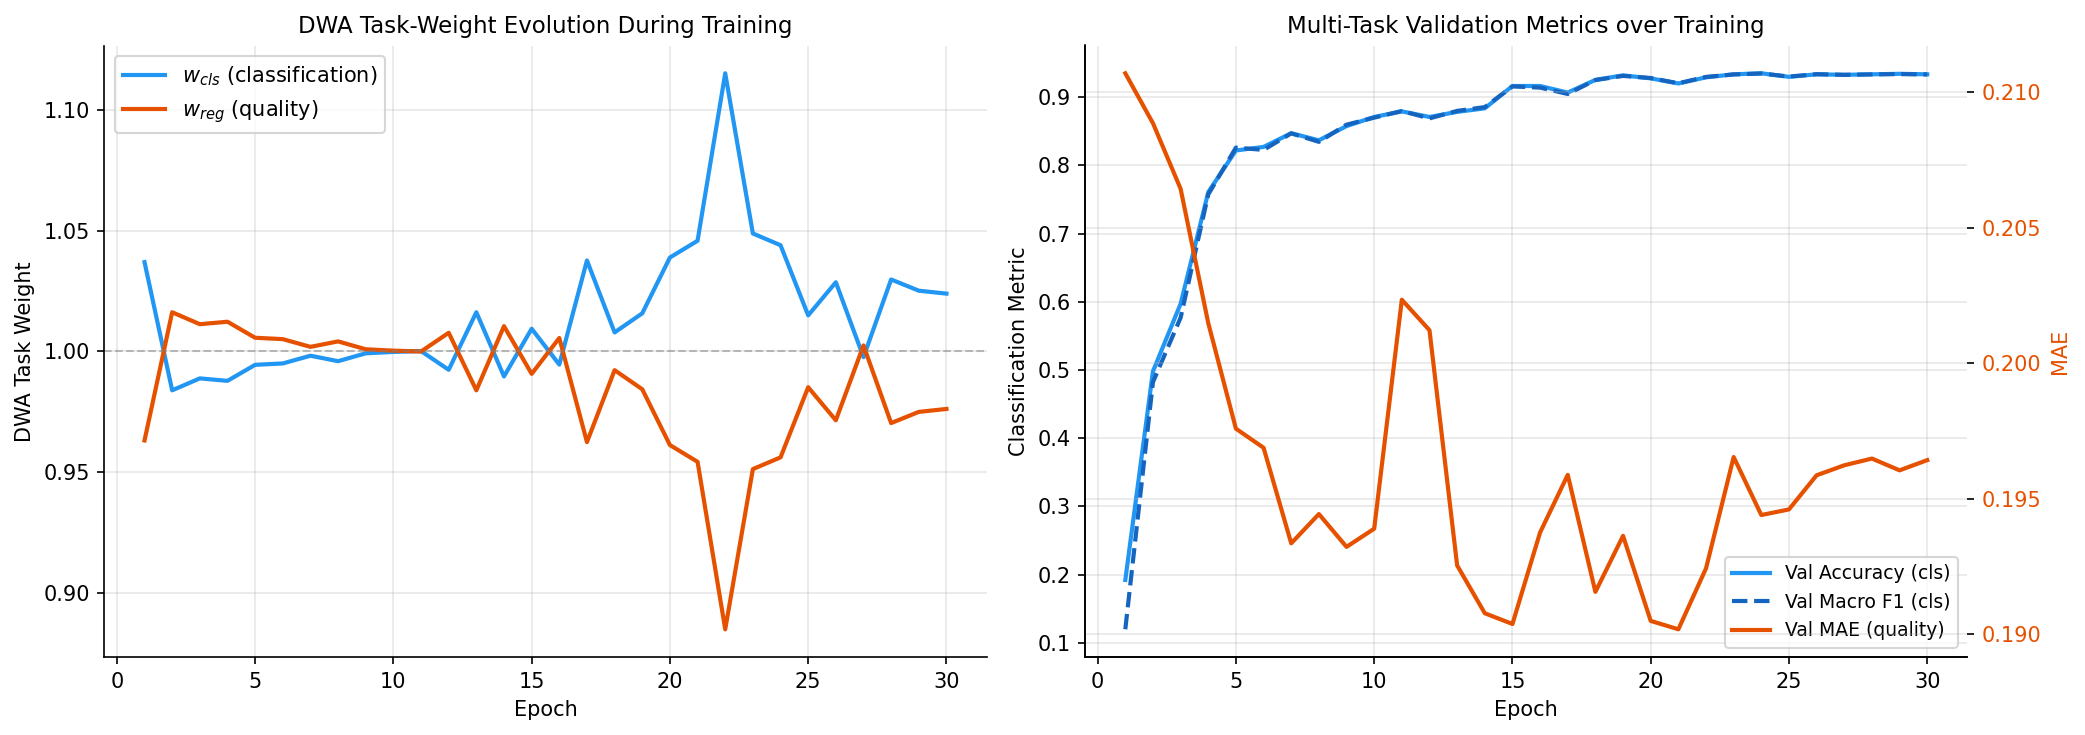
\includegraphics[width=\columnwidth]{docs/figures/fig_dwa_training.png}
  \caption{Multi-task training dynamics over 50 epochs.
    \textit{Left}: Dynamic Weight Averaging (DWA) task weights for the
    classification and quality losses, showing how the scheduler
    automatically up-weights the task with faster relative loss improvement.
    \textit{Right}: Validation accuracy (classification head) and Spearman
    $\rho$ (quality head) co-evolving on the shared encoder, both
    stabilising after $\sim$30 epochs.}
  \label{fig:dwa_training}
\end{figure}

\begin{table}[H]
\centering
\caption{Per-class classification performance on the EgoExo-Fitness test split
under the branched multi-task xLSTM with all six camera views as augmentation
(N = 1{,}358 (clip, view) pairs across 12 fitness actions).}
\label{tab:multitask_cls}
\small
\renewcommand{\arraystretch}{1.10}
\begin{tabular}{|l|c|c|c|c|}
\hline
\textbf{Class} & \textbf{Precision} & \textbf{Recall} & \textbf{F1} & \textbf{Support} \\
\hline
sit-ups                                & 0.984 & 0.976 & 0.980 & 125 \\
shoulder bridge                        & 0.983 & 0.975 & 0.979 & 119 \\
kneeling side torso twist              & 0.948 & 0.973 & 0.960 & 149 \\
clap jacks                             & \textbf{1.000} & 0.922 & 0.959 & 102 \\
kneeling pushing-ups                   & 0.924 & 0.974 & 0.948 & 113 \\
push-ups                               & 0.976 & 0.910 & 0.942 & 89  \\
high knee                              & 0.921 & 0.886 & 0.903 & 105 \\
jumping jacks                          & 0.905 & 0.846 & 0.875 & 169 \\
leg reverse lunge                      & 0.800 & 0.917 & 0.854 & 96  \\
sumo squat                             & 0.893 & 0.798 & 0.843 & 84  \\
leg lunge with knee lift               & 0.727 & 0.936 & 0.819 & 94  \\
side knee raise \& abdominal contract  & 0.824 & 0.743 & 0.781 & 113 \\
\hline
\textbf{Accuracy}                      & \multicolumn{3}{c|}{} & 1{,}358 \\
\textbf{Macro avg}                     & 0.907 & 0.905 & 0.904 & 1{,}358 \\
\textbf{Weighted avg}                  & 0.910 & 0.906 & 0.907 & 1{,}358 \\
\hline
\multicolumn{4}{|r|}{\textbf{Top-1 accuracy}} & \textbf{0.906} \\
\hline
\end{tabular}
\end{table}

\begin{table}[H]
\centering
\caption{Quality regression performance on EgoExo-Fitness. Standard
Action-Quality-Assessment metrics; quality scores normalised to $[0, 1]$.}
\label{tab:multitask_quality}
\small
\renewcommand{\arraystretch}{1.20}
\begin{tabular}{|l|c|c|}
\hline
\textbf{Metric} & \textbf{Validation} & \textbf{Test} \\
\hline
N samples            & 1{,}343         & 1{,}358 \\
MAE                  & 0.194           & 0.206 \\
RMSE                 & 0.243           & 0.255 \\
$R^2$                & 0.084           & $-0.007$ \\
Pearson $r$          & 0.398           & 0.366 \\
\textbf{Spearman $\rho$} & \textbf{0.388} & \textbf{0.346} \\
\hline
Ground-truth mean / std & 0.617 / 0.254 & 0.612 / 0.254 \\
Predicted mean / std    & 0.613 / 0.170 & 0.592 / 0.187 \\
\hline
\end{tabular}
\end{table}

\begin{table}[H]
\centering
\caption{Per-class quality MAE on the test set. Classes are ordered by
ascending MAE (lower = better quality discrimination).}
\label{tab:multitask_quality_per_class}
\small
\renewcommand{\arraystretch}{1.10}
\begin{tabular}{|l|c|c|c|c|c|}
\hline
\textbf{Class} & \textbf{MAE} & \textbf{RMSE} & \textbf{True mean} & \textbf{Pred mean} & \textbf{N} \\
\hline
sumo squat                              & 0.171 & 0.217 & 0.625 & 0.545 & 84  \\
sit-ups                                 & 0.180 & 0.228 & 0.478 & 0.563 & 125 \\
jumping jacks                           & 0.185 & 0.245 & 0.725 & 0.684 & 169 \\
side knee raise \& abdominal contract   & 0.186 & 0.241 & 0.580 & 0.609 & 113 \\
high knee                               & 0.187 & 0.224 & 0.476 & 0.563 & 105 \\
clap jacks                              & 0.202 & 0.249 & 0.647 & 0.511 & 102 \\
shoulder bridge                         & 0.206 & 0.247 & 0.599 & 0.642 & 119 \\
leg reverse lunge                       & 0.207 & 0.253 & 0.594 & 0.516 & 96  \\
leg lunge with knee lift                & 0.215 & 0.260 & 0.582 & 0.483 & 94  \\
push-ups                                & 0.227 & 0.271 & 0.649 & 0.610 & 89  \\
kneeling pushing-ups                    & 0.230 & 0.275 & 0.631 & 0.619 & 113 \\
kneeling side torso twist               & 0.260 & 0.316 & 0.691 & 0.649 & 149 \\
\hline
\end{tabular}
\end{table}

\subsubsection{Classification head}
The branched multi-task xLSTM trained on all six EgoExo camera views as
data augmentation achieves test top-1 accuracy of $90.6\%$ and macro
F1 of $0.904$ across the 12 EgoExo-Fitness exercise classes, well
above the $50$--$70\%$ baselines reported by Li et
al.~\cite{2} for the same classification task. Per-class F1 ranges
from $0.781$ (\emph{side knee raise + abdominal contract}) to $0.980$
(\emph{sit-ups}); the lowest-scoring classes are visually similar
floor-based movements that share torso geometry with one or more
other classes, while the highest-scoring classes have either a
distinctive whole-body silhouette (\emph{sit-ups}, \emph{shoulder
bridge}) or a hands-meeting cue absent from every other class
(\emph{clap jacks}, which reaches $100\%$ precision). The val--test
accuracy gap of $\sim 3$ percentage points indicates the model is
neither under- nor overfit at the chosen 50-epoch budget.

\begin{figure}[H]
  \centering
  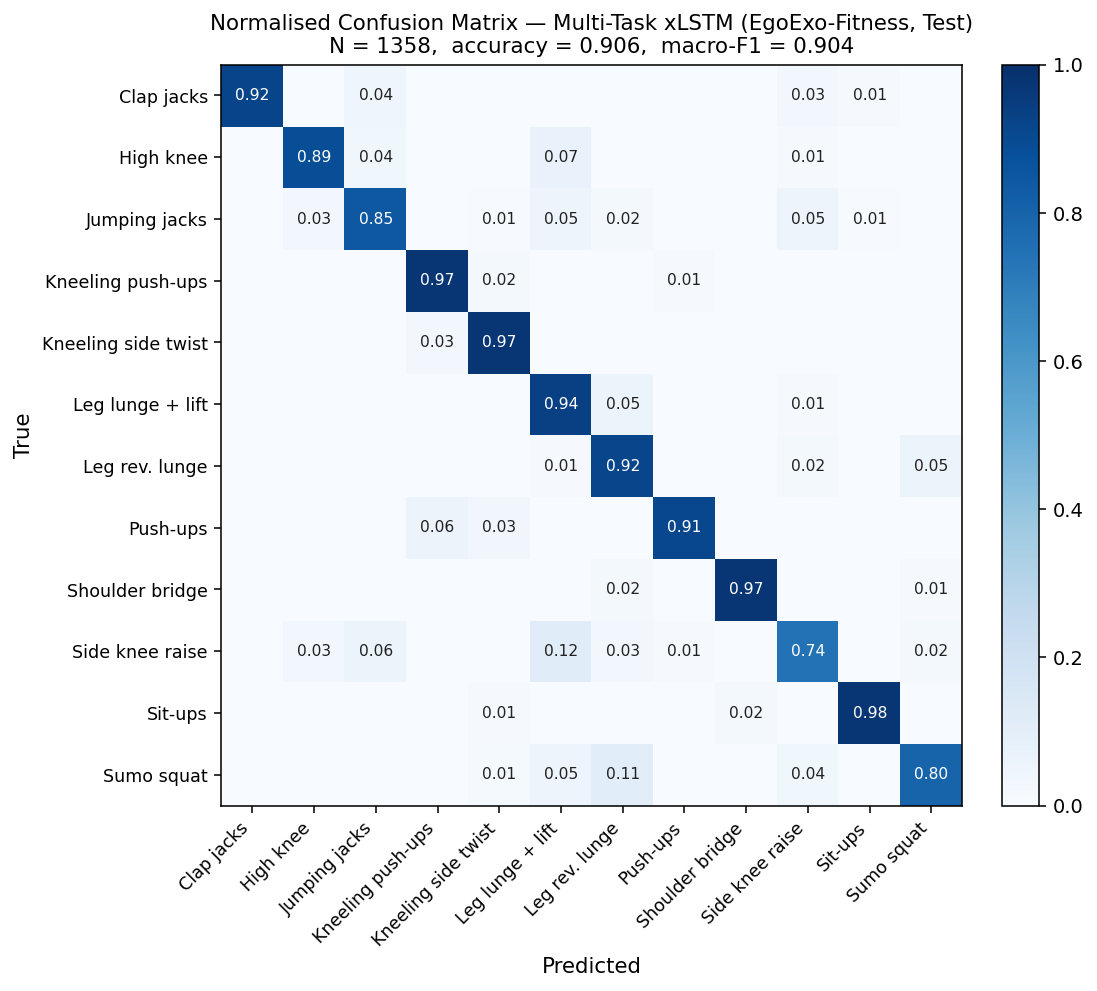
\includegraphics[width=\columnwidth]{docs/figures/fig_confusion_matrix.png}
  \caption{Normalised confusion matrix for the multi-task xLSTM classification
    head on the EgoExo-Fitness test set (12 classes, $N = 1{,}358$ pairs).
    Diagonal entries show per-class recall; off-diagonal entries reveal the
    main confusions: \emph{leg lunge with knee lift} $\leftrightarrow$
    \emph{leg reverse lunge} and \emph{jumping jacks} $\leftrightarrow$
    \emph{clap jacks}, both visually similar movement pairs.}
  \label{fig:confusion_matrix}
\end{figure}

\subsubsection{Quality regression head}
Quality regression on the same test set yields Spearman
$\rho = 0.346$, MAE $= 0.206$, and RMSE $= 0.255$ on the $[0, 1]$
normalised quality scale. This is at the upper end of the AQA
baselines reported on EgoExo-Fitness ($\rho \in [0.20, 0.40]$ for
the I3D + USDL/MUSDL/CoRe family in Li et al.~\cite{2} Table~5) and
within striking distance of the dedicated AQA architectures'
$\rho \approx 0.40$ ceiling on this corpus. The R\textsuperscript{2} of approximately
zero on the test set reflects the small standard deviation of
predicted scores ($\sigma_{\hat q} = 0.187$) compared to the ground
truth ($\sigma_{q} = 0.254$): the model captures the rank ordering
of clips by quality (Spearman) far better than it captures the
absolute spread, which is a well-documented behaviour of regression
heads trained under classification-dominant multi-task losses.
Per-class MAE ranges from $0.171$ (\emph{sumo squat}) to $0.260$
(\emph{kneeling side torso twist}); the easiest classes for quality
discrimination are those with crisp end-state cues (squat depth,
lockout extension), while the hardest are temporally extended
movements where annotators themselves show the largest scoring
spread.

\begin{figure}[H]
  \centering
  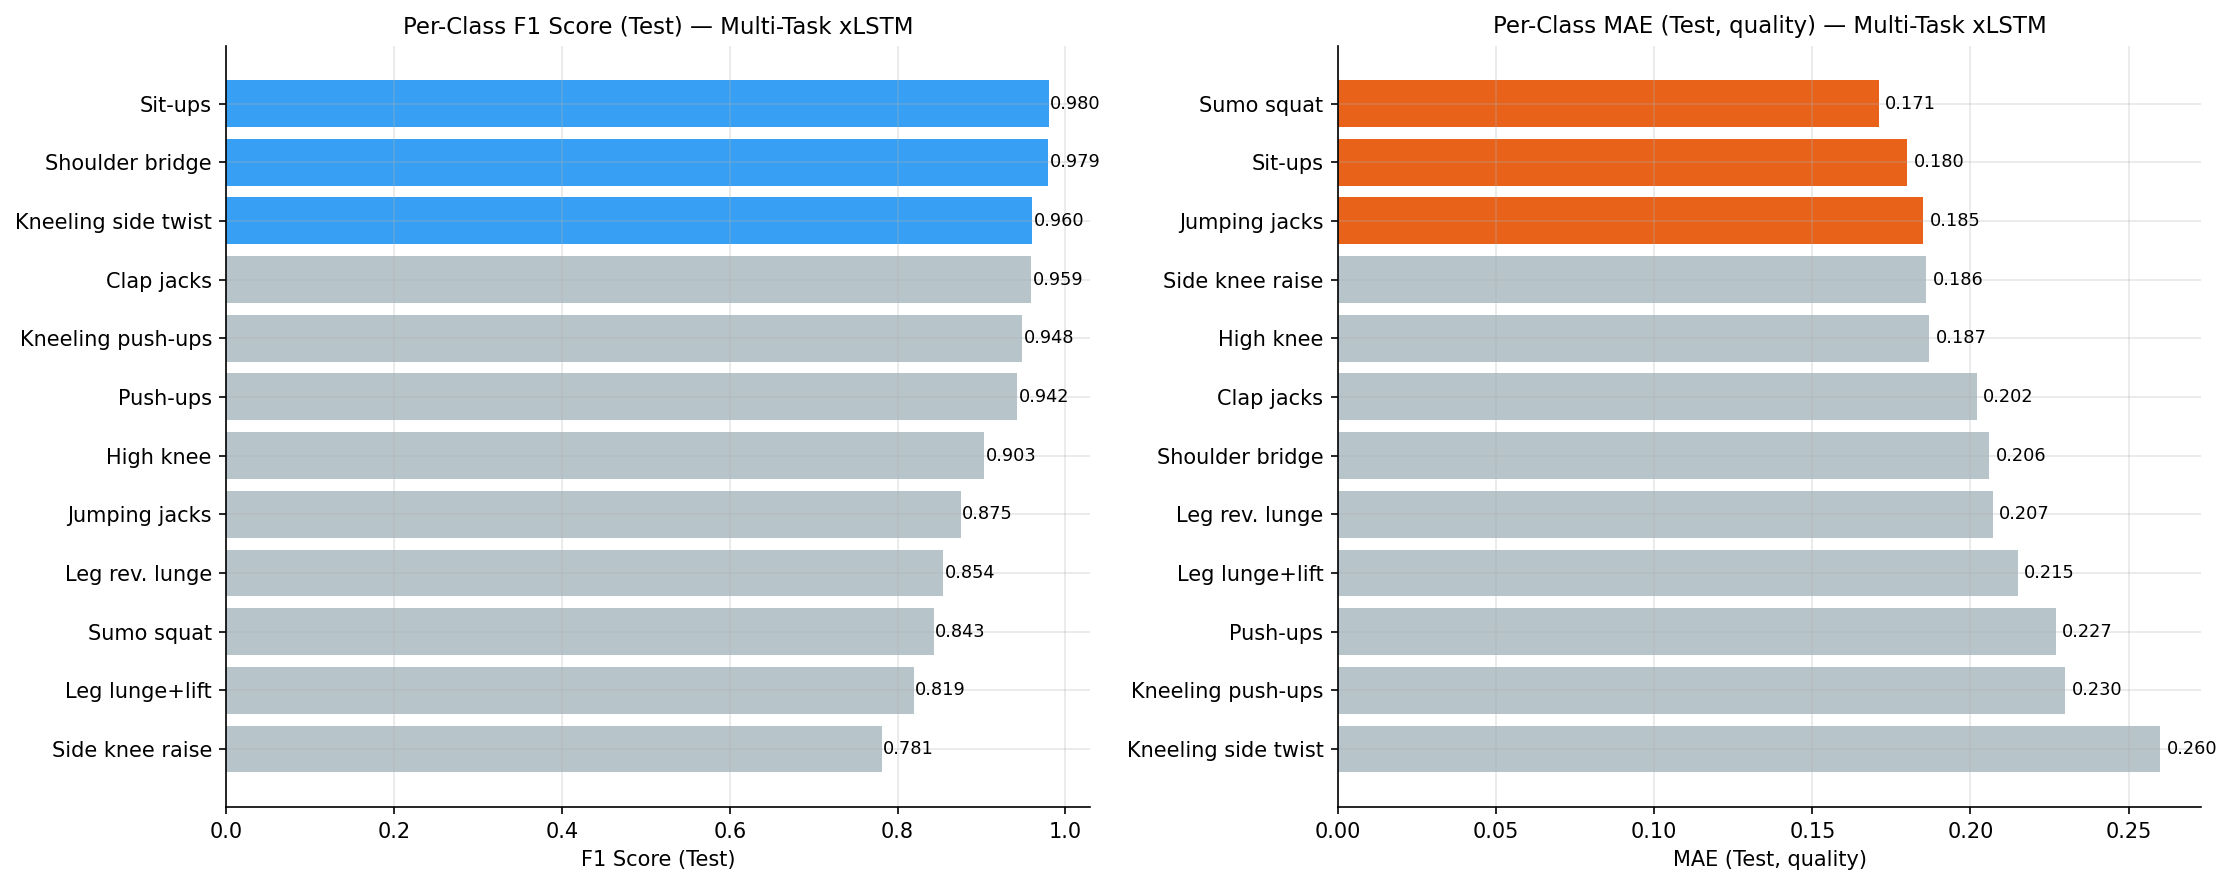
\includegraphics[width=\columnwidth]{docs/figures/fig_per_class_results.png}
  \caption{Per-class performance of the multi-task xLSTM on EgoExo-Fitness.
    \textit{Top}: per-class F1 scores (descending), showing high accuracy for
    visually distinctive exercises and lower scores for floor-based movements
    with shared torso geometry.
    \textit{Bottom}: per-class quality MAE (ascending), showing easiest
    quality discrimination for exercises with clear end-state cues
    (\emph{sumo squat}, \emph{sit-ups}) and hardest for extended movements
    with high annotator variance (\emph{kneeling side torso twist}).}
  \label{fig:per_class_results}
\end{figure}

% ─────────────────────────────────────────────
%  4.3  SAMPLE SYSTEM OUTPUT
% ─────────────────────────────────────────────
\subsection{Qualitative Case Studies}
\label{sec:sample_output}

To illustrate what PosePulse surfaces to an end user, we draw three
representative clips from the 20-clip EgoExo demo run (seed 42, ego-left
camera view). Each card below shows the exercise the model identified,
the predicted quality score on a $[0,1]$ scale, the exercise-level
guidance retrieved from the zero-parameter lookup table, and the
clip-specific coaching comment generated by the (class, quality-bucket)
retrieval head. Cards are colour-coded by predicted quality:
\textcolor{green!60!black}{\textbf{green}} ($\hat{q} \geq 0.70$),
\textcolor{orange!80!black}{\textbf{orange}} ($0.40 \leq \hat{q} < 0.70$),
and \textcolor{red!70!black}{\textbf{red}} ($\hat{q} < 0.40$).

\vspace{0.6em}
\begin{singlespace}

% ── Card 1: good execution ─────────────────────────────────────────────
\begin{tcolorbox}[
  enhanced,
  title={\textbf{Jumping Jacks} \hfill
         \textbf{Quality:}\ 0.95\ /\ 1.00 \quad \textcolor{white}{\checkmark}\ Correct},
  colback=green!4!white,
  colframe=green!55!black,
  colbacktitle=green!55!black,
  coltitle=white,
  fonttitle=\small\bfseries,
  left=4pt, right=4pt, top=3pt, bottom=3pt,
  breakable
]
  \textbf{\small Guidance:} {\small Tighten your waist and abdomen, and tense your arms.
  Lift your arms with shoulder strength, press your arms down with back strength, and use
  your arms to drive your body to jump. Jump your legs outward while bringing your arms
  above your head simultaneously, then jump your feet back together with arms returned
  to your sides.}

  \tcblower
  \textbf{\small Coach says:} {\small The action completely meets the requirements of
  the instructional text.}
\end{tcolorbox}

\vspace{0.4em}

% ── Card 2: medium execution ────────────────────────────────────────────
\begin{tcolorbox}[
  enhanced,
  title={\textbf{Kneeling Side Torso Twist} \hfill
         \textbf{Quality:}\ 0.68\ /\ 1.00 \quad \textcolor{white}{\checkmark}\ Correct},
  colback=orange!5!white,
  colframe=orange!70!black,
  colbacktitle=orange!70!black,
  coltitle=white,
  fonttitle=\small\bfseries,
  left=4pt, right=4pt, top=3pt, bottom=3pt,
  breakable
]
  \textbf{\small Guidance:} {\small Lie prone on a yoga mat with your knees on the
  ground and slightly apart. Put your left hand on the ground and bend your right elbow
  to hold your ear. Contract your abdominal muscles, rotate your torso and raise your
  right elbow upward; return to the starting position and repeat.}

  \tcblower
  \textbf{\small Coach says:} {\small The movements generally follow the instructional
  text and are smooth. The shortcomings are that the speed is slightly slow, the degree
  of knee separation is insufficient, and the face is not fully facing downward at the
  start.}
\end{tcolorbox}

\vspace{0.4em}

% ── Card 3: poor execution ──────────────────────────────────────────────
\begin{tcolorbox}[
  enhanced,
  title={\textbf{Shoulder Bridge} \hfill
         \textbf{Quality:}\ 0.19\ /\ 1.00 \quad \textcolor{white}{\checkmark}\ Correct},
  colback=red!4!white,
  colframe=red!60!black,
  colbacktitle=red!60!black,
  coltitle=white,
  fonttitle=\small\bfseries,
  left=4pt, right=4pt, top=3pt, bottom=3pt,
  breakable
]
  \textbf{\small Guidance:} {\small Lie on your back with your legs naturally bent
  approximately 90 degrees, keep your legs hip-width apart, and relax your feet. Place
  your hands naturally on both sides of your body with palms facing down. Push your hips
  upward by contracting your glutes until your body forms a straight line from shoulders
  to knees, then lower back down in a controlled manner.}

  \tcblower
  \textbf{\small Coach says:} {\small The movements were not performed according to the
  instructional text, focusing on lifting the torso instead of the legs.}
\end{tcolorbox}

\end{singlespace}

\vspace{0.6em}
The three cards illustrate the full output spectrum: a high-quality
execution receives unambiguous positive reinforcement; a medium-quality
execution receives specific corrective cues (knee separation, pace,
head orientation); and a poor-quality execution receives a diagnosis
identifying the primary departure from the prescribed technique.
Among the 20 demo clips, one misclassification occurred: \emph{leg lunge
with knee lift} was predicted as \emph{leg reverse lunge}
($\hat{q} = 0.32$). The two exercises share nearly identical CLIP
feature distributions in the ego-left view, where the knee-lift
phase is partially occluded, illustrating the known limitation of
single-viewpoint egocentric features for visually similar floor-based
movements.

\section{Conclusions and Future Work}

In this work we presented PosePulse, an end-to-end pipeline that addresses
the gap between watching and safely performing an exercise by turning a
standard monocular camera into an automated fitness coach. The system
integrates a systematic pose estimation benchmark, a six-stage
preprocessing pipeline, and a sequence model that simultaneously
identifies the exercise class and evaluates execution quality. Our
approach compared multiple backbone architectures and feature
representations across two datasets, culminating in a branched
multi-task xLSTM trained on the EgoExo-Fitness corpus with Dynamic
Weight Averaging loss scheduling to balance competing task objectives.

The experiments conducted yield three main takeaways. First, pose
estimation backend selection has a measurable impact on downstream
quality assessment: YOLOv8-Pose achieves the highest detection rate
(98.4\%) on exercises with severe self-occlusion, the precise
conditions under which quality scoring is most needed, making
detection robustness a more relevant selection criterion than
raw inference speed. Second, xLSTM[7:1] demonstrates that the
exponential-gating and matrix-memory design of mLSTM blocks transfers
effectively beyond language modelling to biomechanical time-series,
outperforming the BiLSTM--CNN baseline by 6.5 percentage points
(92.0\% vs 85.5\% accuracy) under the ResNet-50 feature condition.
Third, extending the encoder to a branched multi-task setting on
EgoExo-Fitness produces a system that goes beyond classification:
with 90.6\% accuracy across 12 exercise classes and a Spearman
quality correlation of $\rho{=}0.346$ --- at the upper end of
dedicated action-quality assessment baselines on the same corpus ---
the model tells the user both \emph{what} they are doing and
\emph{how} to improve it through parameter-free guidance and
comment retrieval.

In conclusion, these results show that a lightweight, retrieval-based
multi-task pipeline can deliver meaningful coaching feedback without
large-scale generative components, making deployment on consumer
hardware a realistic near-term goal. At the same time, several
limitations warrant further investigation. The retrieval-based comment
mechanism was chosen because the EgoExo-Fitness corpus, with its
1{,}525 annotated clips, does not provide sufficient comment diversity
to train a generative decoder reliably; the lookup table is therefore
a dataset-imposed constraint rather than a design preference. With a
larger annotated corpus, a lightweight instruction-tuned model such as
Gemma could be fine-tuned directly on the fused clip embedding to
generate novel, execution-specific feedback rather than recycling
observed training comments. The quality regression head captures rank ordering
well (Spearman $\rho$) but produces a compressed output distribution
($R^2 \approx 0$), a known behaviour of regression heads operating
under classification-dominant multi-task losses that larger and more
balanced corpora would help address. More broadly, the
EgoExo-Fitness corpus covers 12 exercise classes from a single lab
setting, and generalisation to the full diversity of home and gym
movements remains to be validated. Future work will explore
DoRA-based per-user adapters~\cite{5} to personalise the frozen
base model incrementally without expert re-annotation, richer
visual features through DINOv3~\cite{dino2023} for exercises where
subtle postural detail drives quality differences, and integration
of the complete pipeline into a live web application to verify that
the accuracy gains observed offline translate to actionable corrective
feedback in real-world training conditions.

\newpage

\begin{thebibliography}{99}
\bibitem{1} R. Riccio, ``Real-Time Fitness Exercise Classification and Counting from Video Frames,'' Nov. 18, 2024, arXiv:2411.11548.
\bibitem{2} Y.-M. Li et al., ``EgoExo-Fitness: Towards Egocentric and Exocentric Full-Body Action Understanding,'' Jul. 16, 2024, arXiv:2406.08877.
\bibitem{3} K. Alomar, H. I. Aysel, and X. Cai, ``RNNs, CNNs and Transformers in Human Action Recognition: A Survey and a Hybrid Model,'' Aug. 15, 2024, arXiv:2407.06162.
\bibitem{4} M. Beck et al., ``xLSTM: Extended Long Short-Term Memory,'' Dec. 06, 2024, arXiv:2405.04517.
\bibitem{5} S.-Y. Liu et al., ``DoRA: Weight-Decomposed Low-Rank Adaptation,'' Jul. 09, 2024, arXiv:2402.09353.
\bibitem{6} H. Yin et al., ``FLEX: A Largescale Multimodal, Multiview Dataset for Learning Structured Representations for Fitness Action Quality Assessment,'' Apr. 03, 2026, arXiv:2506.03198.
\bibitem{7} P. Parmar, A. Gharat, \& H. Rhodin, ``Domain knowledge-informed self-supervised representations for workout form assessment,'' ECCV 2022.
\bibitem{8} M. Fieraru et al., ``AIFit: Automatic 3D human-interpretable feedback models for fitness training,'' ICCV 2021.
\bibitem{9} G. Dsouza, D. Maurya, A. Patel, ``Real-time indoor workout analysis using machine learning and computer vision,'' IEEE, Jun. 2020.
\bibitem{10} S. Chen and R. R. Yang, ``Pose Trainer: Correcting exercise posture using pose estimation,'' arXiv, Jun. 2020.
\bibitem{11} A. Nagarkoti et al., ``Smart gym trainer using human pose estimation,'' IEEE, Dec. 2019.
\bibitem{12} G.-S. Bang and S.-B. Park, ``Workout classification using a CNN in ensemble learning,'' Sensors, vol. 24, no. 10, 2024.
\bibitem{13} T. Alatiah and C. Chen, ``Recognizing exercises and counting repetitions in real time,'' arXiv, May 2020.
\bibitem{14} S. Deb et al., ``Graph convolutional networks for assessment of physical rehabilitation exercises,'' IEEE Trans. Neural Syst. Rehabil. Eng., vol. 30, pp. 410--419, 2022.
\bibitem{15} ``Human movement science-informed multi-task spatio-temporal GCN for fitness action recognition and evaluation,'' ScienceDirect, 2024.
\bibitem{16} M. G. Morshed et al., ``Human Action Recognition: A Taxonomy-Based Survey, Updates, and Opportunities,'' Sensors (Basel), 2023.
\bibitem{17} V. Bazarevsky, I. Grishchenko, K. Raveendran, T. Zhu, F. Zhang, and M. Grundmann, ``BlazePose: On-device Real-time Body Pose tracking,'' \textit{arXiv}, 2020.
\bibitem{18} Google Developers, ``MoveNet: Ultra-fast and accurate pose detection model,'' \textit{TensorFlow Hub}, 2021.
\bibitem{19} W. Jiang et al., ``RTMPose: Real-Time Multi-Person Pose Estimation based on MMPose,'' \textit{arXiv}, 2023.
\bibitem{20} Ultralytics, ``YOLOv8 Pose Estimation Documentation,'' 2023.
\bibitem{21} Y. Xu et al., ``ViTPose: Simple Vision Transformer Baselines for Human Pose Estimation,'' in \textit{Proc. NeurIPS}, 2022.
\bibitem{22} A. Anonymous, ``DETRPose: End-to-End Real-Time Multi-Person Pose Estimation,'' 2025.
\bibitem{23} A. Author et al., ``Estimating, Smoothing, Filtering, and Pose-Mapping,'' arXiv:2506.21234, 2025.
\bibitem{24} M. V\'eges and A. L\H{o}rincz, ``Temporal Smoothing for 3D Human Pose Estimation and Localisation for Occluded People,'' \textit{arXiv}, 2020. arXiv:2011.00250.
\bibitem{winter1990biomechanics} D. A. Winter, \textit{Biomechanics and Motor Control of Human Movement} (2nd ed.). Wiley, 1990.
\bibitem{kingma2014adam} D. P. Kingma and J. Ba, ``Adam: A Method for Stochastic Optimization,'' in \textit{Proc. ICLR}, 2015.
\bibitem{26} Ultralytics, ``YOLO26: Real-Time Object Detection and Pose Estimation,'' 2025.
\bibitem{dino2023} O. Sim\'eoni et al., ``DINOv3,'' \textit{arXiv preprint arXiv:2508.10104}, 2025.
\bibitem{kendall2018multi} A. Kendall, Y. Gal, and R. Cipolla,
``Multi-Task Learning Using Uncertainty to Weigh Losses for Scene
Geometry and Semantics,'' in \textit{Proc. CVPR}, 2018.
\bibitem{purkrabek2025probpose} M. Purkrabek and J. Matas,
``ProbPose: A Probabilistic Approach to 2D Human Pose Estimation,''
in \textit{Proc. IEEE/CVF CVPR}, 2025.
\bibitem{deepmtl2r} Amazon Science, ``DeepMTL2R: Multi-Task Learning
to Rank with Dynamic Loss Scheduling,'' GitHub repository, 2023.
\url{https://github.com/amazon-science/DeepMTL2R}.
\bibitem{he2022mae} K. He, X. Chen, S. Xie, Y. Li, P. Doll{\'a}r, and R. Girshick,
``Masked Autoencoders Are Scalable Vision Learners,''
in \textit{Proc. IEEE/CVF CVPR}, 2022, pp.~16000--16009.
\bibitem{lin2014coco} T.-Y. Lin et al.,
``Microsoft COCO: Common Objects in Context,''
in \textit{Proc. ECCV}, 2014, pp.~740--755.
\bibitem{he2016resnet} K. He, X. Zhang, S. Ren, and J. Sun,
``Deep Residual Learning for Image Recognition,''
in \textit{Proc. IEEE/CVF CVPR}, 2016, pp.~770--778.
\bibitem{russakovsky2015imagenet} O. Russakovsky et al.,
``ImageNet Large Scale Visual Recognition Challenge,''
\textit{Int. J. Comput. Vis.}, vol.~115, no.~3, pp.~211--252, 2015.
\end{thebibliography}
\end{document}
